\documentclass[preprint,11pt]{elsarticle}
\usepackage{amsmath,amssymb,amsthm,amsfonts,bm}
\usepackage{graphicx}
\usepackage{array}
\usepackage{algorithm}
\usepackage{algpseudocode}
\usepackage{tikz}
\usepackage{subcaption}
\usetikzlibrary{arrows.meta,positioning,shapes.geometric,fit,calc,decorations.pathreplacing}
\usepackage[hidelinks]{hyperref}
\usepackage{setspace}
\emergencystretch=3em

\newtheorem{theorem}{Theorem}
\newtheorem{lemma}{Lemma}
\newtheorem{proposition}{Proposition}
\newtheorem{corollary}{Corollary}
\theoremstyle{definition}
\newtheorem{definition}{Definition}
\theoremstyle{remark}
\newtheorem{remark}{Remark}
% restated statements in the appendix
\newenvironment{repeattheorem}[1][]{\par\medskip\noindent\textbf{#1.}\ \itshape}{\par\medskip}
\newenvironment{repeatlemma}[1][]{\par\medskip\noindent\textbf{#1.}\ \itshape}{\par\medskip}
\newenvironment{repeatproposition}[1][]{\par\medskip\noindent\textbf{#1.}\ \itshape}{\par\medskip}
\newenvironment{repeatremark}[1][]{\par\medskip\noindent\textbf{#1.}\ \itshape}{\par\medskip}
\newcommand{\up}{\rule{0pt}{2.6ex}}
\newcommand{\down}{\rule[-1.2ex]{0pt}{0pt}}
\newcommand{\Rspread}{R}
\newcommand{\FF}{F}

\journal{Operations Research Perspectives}

\begin{document}

\begin{frontmatter}
\title{Adaptive Influence Minimization via Deferred Frontier Blocking}
\author[a]{Quang-Vinh Dang}
\ead{vinh.dq4@buv.edu.vn}
\author[b]{Dat Le}
\ead{datla@uef.edu.vn}
\author[c]{Minh Ngoc Dinh\corref{cor1}}
\ead{minh.dinh@maeducation.com}
\cortext[cor1]{Corresponding author.}
\affiliation[a]{organization={British University Vietnam},
            city={Hung Yen},
            country={Vietnam}}
\affiliation[b]{organization={Department of Science, Technology, and International Projects, Ho Chi Minh City University of Economics and Finance},
            city={Ho Chi Minh City},
            postcode={700000},
            country={Vietnam}}
\affiliation[c]{organization={Millennia Education},
            city={Ho Chi Minh City},
            country={Vietnam}}

\begin{abstract}
Blocking the spread of a rumor or epidemic that has already started, by removing a few nodes under a fixed budget, is usually posed as a one-shot decision made before the outbreak is observed. We ask whether spending the budget gradually, as the cascade unfolds, can be worse than spending it at once, and how large the benefit can be. We introduce DEFER, a wrapper that turns any one-shot influence minimization planner into an adaptive one: it re-plans every round and blocks a planned node only once the cascade has reached its neighborhood. We prove that the pure-deferral variant is never worse in expectation than the planner it wraps, provided plan replacement passes a held-out test whose residual error we do not bound; that a local rule for early commitment can fail when deferred targets compete for the budget; and that the adaptivity gap of influence minimization is unbounded. With every policy facing the same random cascades, DEFER saves 36 to 97 percent of the spread on the star-of-paths family used in the proof and beats the greedy, re-planning and one-shot integer-programming policies in all 18 settings. On 45 synthetic settings it is significantly better than greedy in 9 and never significantly worse, with gains in large-cascade regimes; on four empirical and synthetic networks, in 5 of 40 settings, with small typical differences. Integer programs over sampled scenarios did not beat greedy or DEFER and ran orders of magnitude slower.
\end{abstract}

\begin{keyword}
influence minimization \sep adaptive optimization \sep misinformation blocking \sep adaptivity gap \sep network optimization
\end{keyword}
\end{frontmatter}

\section{Introduction}\label{sec:intro}

Consider a platform moderator who learns that a false rumor has started spreading from a handful of accounts, or a health authority that has detected a few cases of an infectious disease. Each can suspend a small number of accounts, or quarantine a small number of people, but not many. The standard operations-research treatment asks which targets to pick \emph{now}, and commits the whole budget before anything further is known. Real interventions rarely work this way: within hours or days the moderator sees which accounts the rumor has actually reached, and the authority sees which contacts have actually become infected. The practical question is whether it is better to spend the budget at once or to hold part of it back and spend it where the outbreak actually goes. Holding back is risky, because a cascade can pass through a node before it is blocked, but it also avoids spending budget on targets the cascade never reaches. This paper quantifies that trade-off.

The problem is \emph{influence minimization} (IMIN) \citep{xie2023,xie2024}: given the seeds of a cascade under the independent cascade model and a budget of vertices that can be removed, choose the vertices that minimize the expected final spread. IMIN is the natural complement of influence \emph{maximization} \citep{kempe2003}. Unlike maximization its objective is not supermodular, so greedy selection carries no approximation guarantee, and the problem is NP-hard and hard to approximate \citep{xie2023}. The IMIN algorithms we know of, AdvancedGreedy and GreedyReplace \citep{xie2023,xie2024} and the Sandwich family \citep{wang2024sandwich}, are \emph{one-shot}: the entire budget is spent before the cascade is observed.

\paragraph{What we ask} Two questions follow. Observation-based adaptive blocking has been studied before \citep{shi2019}, but we are not aware of an answer, for IMIN, to either of these. Can adapting to the unfolding cascade ever hurt, relative to the one-shot plan of a given planner? And how large can the benefit of adapting be, in the worst case? A third question is practical: in which networks and regimes does adapting actually pay, and is it worth the added computation compared with solving the one-shot problem exactly?

\paragraph{A numerical illustration} Seed $s$ has four neighbors, each independently reached with probability $0.1$; a reached neighbor starts a private chain of $50$ further vertices that the cascade follows with certainty. With no blocking the expected spread is $20.4$ vertices. With a budget of one block, the best one-shot choice removes one neighbor in advance and leaves an expected spread of $15.3$, because it must protect against a threat that is absent $90\%$ of the time. A policy that waits one round, sees which neighbors were reached, and blocks the first vertex of one reached chain has an expected spread of $3.2$ (Section~\ref{sec:defer-example}).

\paragraph{What we find} Table~\ref{tab:summary} gives the answers in one place, with the sections where each is established. Terms used there: AG and GR are the one-shot planners AdvancedGreedy and GreedyReplace; COMMIT re-plans every round and commits the whole plan at once (no deferral); DEFER-nopush is DEFER without the push-down rule; ILP is an integer linear program. The \emph{saved fraction} of a policy is one minus its total spread divided by the total spread without blocking, computed over the same random cascades for every policy. A comparison is called \emph{significant} when the mean paired difference exceeds twice its standard error.

\begin{table}[h]
\centering
\caption{Summary of results.}\label{tab:summary}
\small
\begin{tabular}{@{}p{0.26\textwidth}p{0.55\textwidth}p{0.11\textwidth}@{}}
\hline
\up Question & Answer & Where \\
\hline
\up Can adapting hurt? & Pure deferral (DEFER-nopush) is never worse in expectation than the planner it wraps, up to a selection-bias caveat. Early commitment by the push-down rule is optimal for a single target but can make DEFER worse than its planner when targets compete for the budget. & Sec.~\ref{sec:defer-theory} \\
How large can the benefit be? & Unbounded. On the star-of-paths family the saving ratio approaches $(1-(1-p)^\Delta)/p$ and the spread ratio grows without limit. In simulation DEFER saves $0.36$--$0.97$ of the spread there and exceeds the best of AG, GR, COMMIT and the one-shot ILP by at least $0.27$ in all 18 settings. & Sec.~\ref{sec:defer-theory}, \ref{sec:exp-sop} \\
Where does it help in practice? & In large-cascade regimes. Over 45 synthetic settings DEFER is significantly better than AG in 9, better than COMMIT in 6, and never significantly worse. On four networks of 2,000 to 9,900 vertices (40 settings) it is significantly better than AG in 5 and never significantly worse, with small typical differences; the largest is 13.9 points at budget 20 on ca-HepTh. & Sec.~\ref{sec:exp-regime}, \ref{sec:defer-experiments}\\
Does solving the sampled problem exactly help? & No. A time-indexed ILP over 48 sampled scenarios, one-shot or staged, did not beat greedy (within $0.02$ of AG in 13 of 19 cells) and ran far slower; the ILP as DEFER's planner matched the ILP alone. & Sec.~\ref{sec:exp-ilp} \\
What does it cost? & DEFER's cost is AG's per-round cost times the number of rounds, which was $2.1$--$4.9\times$ AG's wall-clock time on the four networks. & Sec.~\ref{sec:defer-theory}, \ref{sec:complexity-comparison}\\
\hline
\end{tabular}
\end{table}

\paragraph{Contributions} (i) DEFER, a wrapper that makes any one-shot planner adaptive (Section~\ref{sec:defer}). (ii) Three theoretical results on when adapting is safe and how much it can help: weak dominance of pure deferral, a local optimality result for push-down together with a counterexample showing it does not extend, and an unbounded adaptivity gap with an explicit construction (Section~\ref{sec:defer-theory}). (iii) An empirical study designed to show where the theory bites: the proof's own family, a grid of synthetic regimes with paired comparisons, empirical networks, and exact integer-programming baselines (Section~\ref{sec:experiments}). The study reports the settings in which DEFER does not help as well as those in which it does.

\paragraph{Roadmap} Section~\ref{sec:related} reviews related work and Section~\ref{sec:prelim} fixes the model. Section~\ref{sec:defer} presents DEFER, first the algorithm, then a worked example that shows the effect in numbers, then the guarantees, each preceded by a plain-language statement of what it says. Section~\ref{sec:experiments} reports the experiments and Section~\ref{sec:discussion} discusses them and the limitations. Proofs and further details are in the appendices.

\section{Related Work}\label{sec:related}

DEFER touches four lines of work: influence maximization and its adaptive variants, influence minimization and blocking, epidemic control and network interdiction, and stochastic optimization with recourse. Table~\ref{tab:related} summarizes how this paper relates to each, and the subsections give the details.

\begin{table}[h]
\centering
\caption{Positioning of this paper. ``Gap'' is the adaptivity gap, the loss from committing in advance.}\label{tab:related}
\small
\begin{tabular}{@{}>{\raggedright\arraybackslash}p{0.2\textwidth}>{\raggedright\arraybackslash}p{0.17\textwidth}>{\raggedright\arraybackslash}p{0.17\textwidth}>{\raggedright\arraybackslash}p{0.18\textwidth}>{\raggedright\arraybackslash}p{0.22\textwidth}@{}}
\hline
\up Line of work & Action & Timing & Known & This paper \\
\hline
\up Influence maximization, adaptive & add seeds & before or while the cascade runs & submodular structure, bounded gap & removes vertices; objective not supermodular; gap unbounded \\
One-shot influence minimization & remove vertices or edges & before the cascade is observed & NP-hard; greedy and sandwich heuristics & wraps these planners \\
Adaptive influence blocking & immunize nodes & after observing the spread & approximation guarantees \citep{shi2019} & not compared (Section~\ref{sec:conclusion}) \\
Immunization and vaccination & vaccinate nodes & mostly fixed in advance & heuristics and spectral surrogates & acts on the realized cascade \\
Stochastic network interdiction & remove arcs & before the opponent moves & exact and decomposition methods & sample-average ILP baseline (Section~\ref{sec:exp-ilp}) \\
\hline
\end{tabular}
\end{table}

\subsection{Influence maximization and adaptive seeding}

Influence maximization asks for the seed set that maximizes the expected spread of a cascade \citep{kempe2003}. Under the independent cascade model its objective is monotone and submodular, so greedy selection has a $(1-1/e)$ guarantee, and much of the later literature is about evaluating the objective faster: lazy evaluation \citep{leskovec2007b} and reverse-reachability sampling with near-linear running time \citep{borgs2014,tang2014}; \citet{li2018} survey the area. Evaluating the spread of a fixed seed set is itself \#P-hard \citep{chen2010}, which is why these methods estimate it by sampling.

Adaptive versions let later choices depend on what has been observed. \citet{golovinkrause2011} give the adaptive-submodularity framework for greedy policies, \citet{seemansinger2013} study two-stage adaptive seeding, \citet{tong2017} re-plan as the network changes, \citet{sun2018} select seeds over several rounds of diffusion, and \citet{yuan2017} study adaptive selection with partial feedback. In these problems an action adds seeds to a cascade that the decision maker wants to grow, and the objective keeps a submodular structure that limits how much adaptivity can help: for stochastic monotone submodular maximization the adaptivity gap is bounded by a constant \citep{asadpournazerzadeh2016}, following the analysis of stochastic knapsack by \citet{deangoemansvondrak2008}. DEFER's setting is the opposite. Its actions remove vertices from a cascade that the decision maker wants to contain, the objective is not supermodular \citep{xie2023}, and Theorem~\ref{thm:adaptivity-gap} shows that the adaptivity gap is unbounded.

\subsection{Influence minimization and blocking}

\citet{xie2023} introduce IMIN, prove NP-hardness and inapproximability, and give AdvancedGreedy and GreedyReplace, extended in \citet{xie2024}. \citet{wang2024sandwich} give the Sandwich lower/upper-bound family and \citet{xiang2024} a pertinence-constrained variant. Earlier work removes links or nodes, or counter-seeds a competing campaign: \citet{kimura2008} block links to minimize the spread of contamination; \citet{budak2011} counter-seed a rival campaign under independent cascade and \citet{he2012} under competitive linear threshold; \citet{nguyen2012}, \citet{wang2013blocking} and \citet{yan2020} study node-removal and blocker problems; \citet{fan2013} add a removal-cost budget; and \citet{kuhlman2013} study edge removal against simple and complex contagion. \citet{tong2012} and \citet{khalil2014} modify the network topology to change the outcome of a diffusion process. \citet{wang2016drimux}, \citet{tong2018} and \citet{farajtabar2017} consider dynamic, multi-campaign or learned settings, and \citet{zareie2021} survey misinformation limitation. Apart from one work discussed next, these methods choose their interventions before the process is observed.

The exception is close to ours. \citet{shi2019} propose adaptive influence blocking, in which the nodes to immunize are chosen using observations of the spread so far, and give algorithms with approximation guarantees. We have not implemented or compared with their algorithms. What this paper adds is a different set of questions and results: a wrapper that makes \emph{any} one-shot planner adaptive, with a dominance guarantee relative to that planner (Theorem~\ref{thm:defer-dominates}); a natural early-commitment rule, push-down, that is optimal for one target but can fail when targets compete for the budget (Remark~\ref{rem:pushdown-counterexample}); an unbounded adaptivity gap for IMIN; and an empirical study of the regimes in which adapting helps.

\subsection{Epidemic control on networks}

In network epidemiology the corresponding actions are immunization and vaccination. \citet{pastor2002} study immunization of scale-free networks, and \citet{cohen2003} propose acquaintance immunization, which needs no global knowledge of the network. \citet{preciado2014} allocate protection resources against spreading processes by optimizing a spectral measure of the network, and \citet{li2024} quantify the benefit of customized vaccination strategies with a network-based optimization model. These approaches fix the allocation before the outbreak or optimize a spectral surrogate of its growth; DEFER instead acts on the realized cascade.

\subsection{Network interdiction and optimization under uncertainty}

Network interdiction chooses arcs or nodes to remove so as to degrade an opponent's objective. \citet{smith2020} survey the models and algorithms, and \citet{cormican1998} study the stochastic version in which network data are uncertain when the interdictor acts. The staged-decision view is standard in stochastic programming: the decision at each stage may depend only on the information revealed so far (non-anticipativity), and models are solved over a scenario tree \citep{birge2011} or over sampled scenarios by sample average approximation \citep{kleywegt2002}. Section~\ref{sec:exp-ilp} builds a time-indexed integer program of this kind as a baseline. Staged choices in a network under uncertainty also appear outside cascades, for example as optimal paths in multi-stage stochastic decision networks \citep{roohnavazfar2019}. The sequential decision problem of Definition~\ref{def:adaptive-imin} is the kind of problem that approximate dynamic programming addresses, whose applications in defence operations research are reviewed by \citet{rempel2021}; DEFER is a heuristic policy for it with a worst-case comparison against one-shot plans, not an approximate dynamic program. Adaptivity gaps measure the loss from committing in advance in stochastic problems \citep{deangoemansvondrak2008,gupta2016}. DEFER re-solves its planning problem every round and commits only the exposed part of the plan, which is the pattern of receding-horizon control \citep{mayne2000}; its default planner uses dominator trees \citep{lengauer1979} on sampled live-edge subgraphs, as AdvancedGreedy does.

\section{Preliminaries}\label{sec:prelim}
\subsection{The independent cascade model}\label{sec:ic-model}

$G=(V,E)$ is a directed graph,
$n=|V|$, $m=|E|$, with edge probabilities $p:E\to(0,1]$. A live-edge
realization $\omega\in\{0,1\}^E$ is drawn with
$\Pr[\omega]=\prod_{e}p_e^{\omega_e}(1-p_e)^{1-\omega_e}$. For a seed set
$S\subseteq V$ and blocked set $B\subseteq V\setminus S$, write
$G_B=G[V\setminus B]$ and let $\Rspread(\omega,B)\subseteq V\setminus B$ be
the set of vertices reachable from $S$ using only live edges of $G_B$. The
\emph{expected spread} is
\begin{equation}\label{eq:spread}
\FF(B)\;=\;\mathbb E_\omega\bigl[\,|\Rspread(\omega,B)\setminus S|\,\bigr].
\end{equation}

\subsection{Problem formalization}\label{sec:formalization}

\begin{definition}[IMIN, one-shot]\label{def:imin}
Given $G$, $p$, seed set $S$, and budget $b\in\mathbb N$, the
\emph{influence minimization} (IMIN) problem is
\begin{equation}\label{eq:imin}
\min_{B\subseteq V\setminus S}\ \FF(B)
\qquad\text{subject to}\qquad
|B|\le b.
\end{equation}
\end{definition}

\noindent \citet{xie2023} show Problem~\eqref{eq:imin} is NP-hard and hard
to approximate within any constant factor unless P$=$NP, and that $\FF$ is
not supermodular in $B$ under the IC model, so the greedy
$(1-1/e)$-guarantee available for influence \emph{maximization}
\citep{kempe2003} does not transfer.

To formalize the adaptive variant, let a \emph{history} up to round $t$ be
$h_t=(N_0,N_1,\dots,N_t)$, the sequence of newly activated sets observed so
far (full-adoption feedback: which vertices activate each round, not which
live edges carried the activation). Let $\mathcal H$ denote the set of all
histories of any length.

\begin{definition}[Adaptive policy]\label{def:policy}
An \emph{adaptive blocking policy} is a function
$\pi:\mathcal H\to 2^V$ mapping each history $h_t$ to a set of
not-yet-activated, not-yet-blocked vertices to additionally block in round
$t+1$, subject to $\sum_{t}|\pi(h_t)|\le b$ over the run of the cascade.
Write $\sigma(\pi)$ for the (random) final spread beyond $S$ that results
from running the cascade under policy $\pi$.
\end{definition}

\begin{definition}[IMIN, adaptive]\label{def:adaptive-imin}
Given $G$, $p$, $S$, and budget $b$, the \emph{adaptive} IMIN problem is
\begin{equation}\label{eq:adaptive-imin}
\min_{\pi}\ \mathbb E\bigl[\sigma(\pi)\bigr]
\qquad\text{subject to}\qquad
\textstyle\sum_t|\pi(h_t)|\le b\ \text{a.s.}
\end{equation}
A one-shot policy is the special case $\pi(h_0)=B$ for a fixed
$B$ with $|B|\le b$ and $\pi(h_t)=\varnothing$ for $t\ge1$, so
Problem~\eqref{eq:imin} is exactly Problem~\eqref{eq:adaptive-imin}
restricted to one-shot policies, and
$\min_\pi\mathbb E[\sigma(\pi)]\le\min_{|B|\le b}\FF(B)$ trivially, since
every one-shot policy is a feasible (adaptive) policy. The
\emph{adaptivity gap} of an instance is the ratio of the right-hand side to
the left-hand side of this inequality; Theorem~\ref{thm:adaptivity-gap}
shows this gap is unbounded.
\end{definition}

DEFER (Section~\ref{sec:defer}) is a construction of a specific policy $\pi_{\mathrm{DEFER}}$, parameterized by a choice of one-shot planner $\mathcal P$, that is feasible for Problem~\eqref{eq:adaptive-imin} and provably no worse than $\mathcal P$'s own one-shot value in its pure-deferral form (Theorem~\ref{thm:defer-dominates}). Table~\ref{tab:notation} lists the notation.

\begin{table}[h]
\centering
\caption{Notation.}\label{tab:notation}
\small
\begin{tabular}{@{}ll@{}}
\hline
\up Symbol & Meaning \\
\hline
\up $G=(V,E)$, $n$, $m$ & graph, vertex count, edge count \\
$p:E\to(0,1]$ & independent-cascade edge probabilities \\
$S$, $B$, $b$ & seed set, blocked set, blocking budget \\
$\omega$, $\Rspread(\omega,B)$ & live-edge realization, reachable set under $\omega$ with $B$ removed \\
$\FF(B)$ & expected spread with blocking set $B$ (Eq.~\ref{eq:spread}) \\
$F_t$, $A_t$, $N_t$ & round-$t$ frontier, active set, newly activated set \\
$P_t$, $L$, $C_t$ & round-$t$ plan, uncommitted leftover, vertices committed this round \\
$q_v$, $c_v$, $\lambda_t$ & exposure probability, child count, shadow price of a budget unit \\
\down $\mathcal P$ & one-shot planner wrapped by DEFER \\
\hline
\end{tabular}
\end{table}
\section{DEFER: Adaptive Influence Minimization by Deferred Frontier Blocking}\label{sec:defer}

\subsection{Algorithm}\label{sec:defer-algo}

DEFER wraps a one-shot planner $\mathcal P$ (any IMIN algorithm; by default
a dominator-tree greedy planner with isolation moves). At each round it
re-plans on the currently reachable region, keeps whichever of the new plan
and the previous round's uncommitted leftover looks better on freshly drawn
samples (\emph{plan protection}), and commits only the fraction of the plan
that is both exposed to the current frontier and passes a push-down test.

\begin{algorithm}[h]
\caption{DEFER}\label{alg:defer}
\begin{algorithmic}[1]
\Require graph $G$, probabilities $p$, seeds $S$, budget $b$, sample size
  $\theta$, one-shot planner $\mathcal P$
\State $A_0\gets S$, $B_0\gets\varnothing$, $F_0\gets S$, $L\gets\varnothing$ (uncommitted leftover)
\For{$t=0,1,2,\dots$ while the cascade is alive and $|B_t|<b$}
  \State $b_t\gets b-|B_t|$
  \State draw $\theta$ live-edge subgraphs reachable from $F_t$ avoiding $A_t\cup B_t$
  \State $P'\gets\mathcal P(\text{seeds}=F_t,\ \text{forbidden}=A_t\cup B_t,\ \text{budget}=b_t)$ on the samples
  \State draw a fresh, held-out set of $\theta$ live-edge subgraphs (disjoint from those used to compute $P'$)
  \State $\hat d\gets$ sample-average saving of $P'$ minus sample-average saving of $L$ on the held-out draws; $\widehat{\mathrm{se}}\gets$ their standard error
  \If{$\hat d>\widehat{\mathrm{se}}$} \Comment{plan protection: swap only if the improvement exceeds one held-out standard error}
    \State $P_t\gets P'$
  \Else
    \State $P_t\gets L$
  \EndIf
  \State $X_t\gets$ inactive, unblocked out-neighbors of $F_t$
  \State $\lambda_t\gets$ smallest marginal saving among the picks of $P_t$ (0 if $P_t$ does not exhaust $b_t$)
  \For{$v\in P_t\cap X_t$}\label{alg:pushdown-start}
    \State $q_v\gets 1-\prod_{u\in F_t}(1-p(u,v))$; $c_v\gets$ inactive unblocked out-degree of $v$
    \If{$\lambda_t=0$ \textbf{or} $q_v\,(c_v+1/\lambda_t)\ge 1$} \Comment{push-down rule, Lemma~\ref{lem:pushdown} (myopic, no budget-contention guarantee -- Remark~\ref{rem:pushdown-counterexample})}
      \State block $v$ now
    \EndIf
  \EndFor\label{alg:pushdown-end}
  \State $L\gets P_t\setminus(\text{blocked this round})$
  \State observe $N_{t+1}$; update $A_{t+1},F_{t+1}$
\EndFor
\end{algorithmic}
\end{algorithm}

The push-down rule compares spending one budget unit on an exposed node $v$
now against waiting one round and, if $v$ activates (probability $q_v$),
protecting its $c_v$ children instead while losing $v$ itself. When the
planner is deterministic given the samples and no new information arrives,
DEFER reduces to lazily committing the one-shot planner's own plan
(Lemma~\ref{lem:defer-free}); the two ablations used in
Section~\ref{sec:experiments} are COMMIT (same loop, but the whole plan is
committed every round) and the one-shot planners run without any wrapper.
Figure~\ref{fig:defer-flow} shows the round-by-round control flow this
paragraph and Algorithm~\ref{alg:defer} describe, and Figure~\ref{fig:timeline} shows its effect on one small cascade.

\begin{figure}[h]
\centering
\begin{subfigure}[t]{0.32\textwidth}
\centering
\resizebox{\linewidth}{!}{%
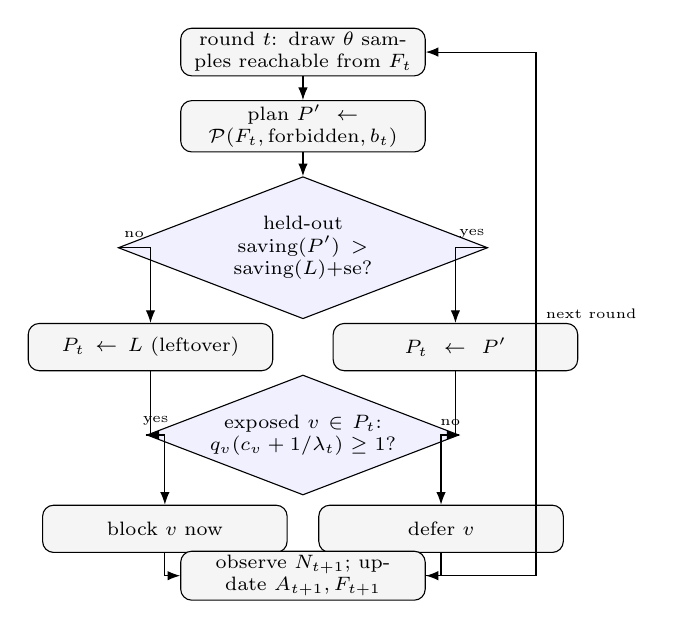
\begin{tikzpicture}[
  node distance=3mm and 8mm,
  box/.style={draw, rounded corners, align=center, fill=gray!8, font=\scriptsize, text width=30mm, minimum height=6mm, inner sep=1.5pt},
  dec/.style={draw, diamond, aspect=2.6, align=center, fill=blue!6, font=\scriptsize, text width=25mm, inner sep=0.5pt},
  arr/.style={-{Latex[length=1.6mm]}}
]
\node[box] (draw) {round $t$: draw $\theta$ samples reachable from $F_t$};
\node[box, below=of draw] (plan) {plan $P'\gets\mathcal P(F_t,\text{forbidden},b_t)$};
\node[dec, below=of plan] (protect) {held-out saving$(P')>$ saving$(L)+$se?};
\node[box, below left=5mm and -8mm of protect] (keepold) {$P_t\gets L$ (leftover)};
\node[box, below right=5mm and -8mm of protect] (keepnew) {$P_t\gets P'$};
\node[dec, below=7mm of protect] (push) {exposed $v\in P_t$: $q_v(c_v+1/\lambda_t)\ge1$?};
\node[box, below left=5mm and -8mm of push] (commitnow) {block $v$ now};
\node[box, below right=5mm and -8mm of push] (defer) {defer $v$};
\node[box, below=7mm of push] (obs) {observe $N_{t+1}$; update $A_{t+1},F_{t+1}$};
\draw[arr] (draw) -- (plan);
\draw[arr] (plan) -- (protect);
\draw[arr] (protect) -| node[near start, above, font=\tiny]{no} (keepold);
\draw[arr] (protect) -| node[near start, above, font=\tiny]{yes} (keepnew);
\draw[arr] (keepold) |- (push);
\draw[arr] (keepnew) |- (push);
\draw[arr] (push) -| node[near start, above, font=\tiny]{yes} (commitnow);
\draw[arr] (push) -| node[near start, above, font=\tiny]{no} (defer);
\draw[arr] (commitnow) |- (obs);
\draw[arr] (defer) |- (obs);
\draw[arr] (obs.east) -- ++(14mm,0) |- node[pos=0.25, right, font=\tiny]{next round} (draw.east);
\end{tikzpicture}}
\caption{DEFER's per-round control flow}
\label{fig:defer-flow}
\end{subfigure}%
\hfill
\begin{subfigure}[t]{0.64\textwidth}
\centering
\resizebox{\linewidth}{!}{%
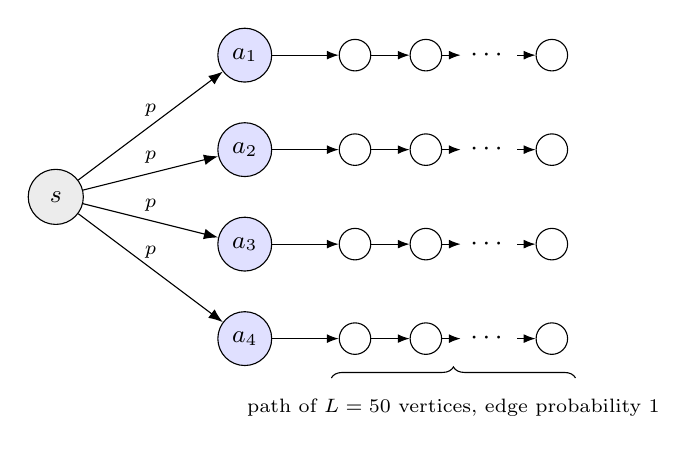
\begin{tikzpicture}[
  seed/.style={draw, circle, fill=gray!15, minimum size=7mm, font=\small},
  gw/.style={draw, circle, fill=blue!12, minimum size=6mm, font=\small},
  pv/.style={draw, circle, fill=white, minimum size=4mm, font=\scriptsize},
  edgelab/.style={font=\scriptsize, above}
]
\node[seed] (s) at (0,0) {$s$};
\foreach \i/\y in {1/1.8,2/0.6,3/-0.6,4/-1.8} {
  \node[gw] (a\i) at (2.4,\y) {$a_{\i}$};
  \draw[-{Latex[length=1.8mm]}] (s) -- node[edgelab]{$p$} (a\i);
  \node[pv] (v\i a) at (3.8,\y) {};
  \node[pv] (v\i b) at (4.7,\y) {};
  \node (dots\i) at (5.5,\y) {$\cdots$};
  \node[pv] (v\i c) at (6.3,\y) {};
  \draw[-{Latex[length=1.5mm]}] (a\i) -- (v\i a);
  \draw[-{Latex[length=1.5mm]}] (v\i a) -- (v\i b);
  \draw[-{Latex[length=1.5mm]}] (v\i b) -- (dots\i);
  \draw[-{Latex[length=1.5mm]}] (dots\i) -- (v\i c);
}
\draw[decorate, decoration={brace, amplitude=4pt}] (3.5,-2.3) -- (6.6,-2.3)
  node[midway, below=4pt, font=\scriptsize]{path of $L=50$ vertices, edge probability $1$};
\end{tikzpicture}}
\caption{The star-of-paths instance behind Theorem~\ref{thm:adaptivity-gap}}
\label{fig:star-of-paths}
\end{subfigure}

\caption{DEFER's control flow, and the star-of-paths worked-example instance. (a) Plan protection (top decision) chooses between the new plan and the
leftover $L$ using a fresh held-out sample; push-down (bottom decision)
then decides, for each planned vertex exposed to the frontier, whether to
commit it now or defer it to a child (Lemma~\ref{lem:pushdown}). (b) Each
of the $\Delta=4$ gateways $a_i$ activates independently with probability
$p=0.1$ from seed $s$ and, if live, deterministically propagates down its
own private length-$L$ path. A one-shot policy commits before observing
which gateways activate; DEFER waits one round, observes $N_1$, and
blocks the first path vertex of one confirmed-live branch (the gateway
itself can no longer be blocked once activated).}
\end{figure}


\begin{figure}[t]
\centering
\resizebox{\textwidth}{!}{%
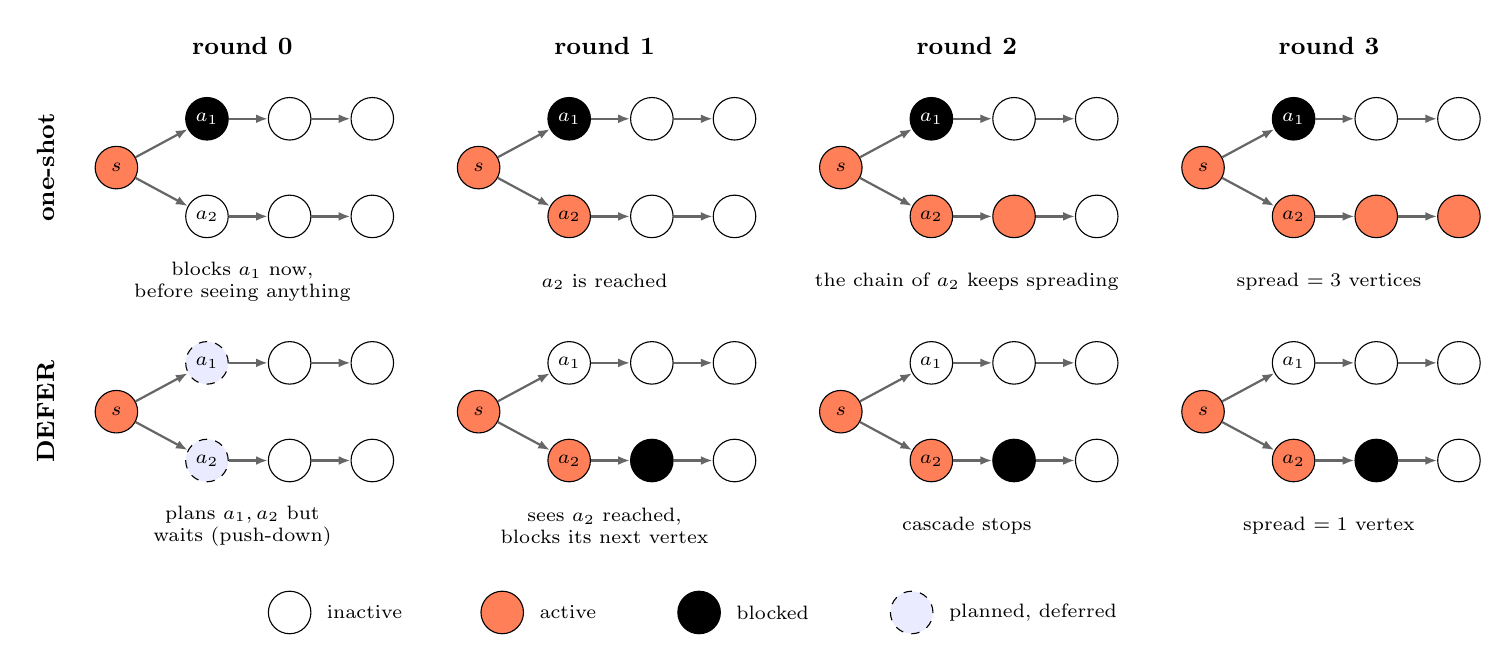
\begin{tikzpicture}[
  n/.style={circle,draw,minimum size=5.4mm,inner sep=0pt,font=\scriptsize},
  ni/.style={n,fill=white}, na/.style={n,fill=red!55!orange!65}, nb/.style={n,fill=black,text=white}, nd/.style={n,dashed,fill=blue!8},
  e/.style={-{Latex[length=1.5mm]},gray!80!black,thick}, lab/.style={font=\scriptsize}, ttl/.style={font=\small\bfseries}]
\newcommand{\mini}[9]{\begin{scope}[shift={(#1,#2)}]
  \node[#3] (s) at (0,0) {$s$};
  \node[#4] (a) at (1.15,0.62) {$a_1$};
  \node[#5] (b) at (1.15,-0.62) {$a_2$};
  \node[#6] (c) at (2.2,0.62) {};
  \node[#7] (d) at (3.25,0.62) {};
  \node[#8] (f) at (2.2,-0.62) {};
  \node[#9] (g) at (3.25,-0.62) {};
  \draw[e] (s)--(a); \draw[e] (s)--(b); \draw[e] (a)--(c); \draw[e] (c)--(d); \draw[e] (b)--(f); \draw[e] (f)--(g);
  \end{scope}}
\foreach \t/\x in {0/0,1/4.6,2/9.2,3/13.8} { \node[ttl] at (\x+1.6,1.55) {round \t}; }
\node[ttl,rotate=90] at (-0.9,0) {one-shot}; \node[ttl,rotate=90] at (-0.9,-3.1) {DEFER};
% one-shot row
\mini{0}{0}{na}{nb}{ni}{ni}{ni}{ni}{ni}
\mini{4.6}{0}{na}{nb}{na}{ni}{ni}{ni}{ni}
\mini{9.2}{0}{na}{nb}{na}{ni}{ni}{na}{ni}
\mini{13.8}{0}{na}{nb}{na}{ni}{ni}{na}{na}
\node[lab,align=center] at (1.6,-1.45) {blocks $a_1$ now,\\ before seeing anything};
\node[lab,align=center] at (6.2,-1.45) {$a_2$ is reached};
\node[lab,align=center] at (10.8,-1.45) {the chain of $a_2$ keeps spreading};
\node[lab,align=center] at (15.4,-1.45) {spread $=3$ vertices};
% DEFER row
\mini{0}{-3.1}{na}{nd}{nd}{ni}{ni}{ni}{ni}
\mini{4.6}{-3.1}{na}{ni}{na}{ni}{ni}{nb}{ni}
\mini{9.2}{-3.1}{na}{ni}{na}{ni}{ni}{nb}{ni}
\mini{13.8}{-3.1}{na}{ni}{na}{ni}{ni}{nb}{ni}
\node[lab,align=center] at (1.6,-4.55) {plans $a_1,a_2$ but\\ waits (push-down)};
\node[lab,align=center] at (6.2,-4.55) {sees $a_2$ reached,\\ blocks its next vertex};
\node[lab,align=center] at (10.8,-4.55) {cascade stops};
\node[lab,align=center] at (15.4,-4.55) {spread $=1$ vertex};
% legend
\node[ni] at (2.2,-5.65) {}; \node[lab,anchor=west] at (2.55,-5.65) {inactive};
\node[na] at (4.9,-5.65) {}; \node[lab,anchor=west] at (5.25,-5.65) {active};
\node[nb] at (7.4,-5.65) {}; \node[lab,anchor=west] at (7.75,-5.65) {blocked};
\node[nd] at (10.1,-5.65) {}; \node[lab,anchor=west] at (10.45,-5.65) {planned, deferred};
\end{tikzpicture}}
\caption{One realization of a small star-of-paths instance with a budget of one block. Gateway $a_2$ becomes active and $a_1$ does not. The one-shot policy must commit at round $0$ and spends its block on $a_1$, which would have stayed inactive, so the chain behind $a_2$ spreads. DEFER keeps its plan uncommitted, observes that $a_2$ was reached, and blocks the first vertex behind it.}\label{fig:timeline}
\end{figure}

\subsection{Worked example}\label{sec:defer-example}

Before stating the formal results of Section~\ref{sec:defer-theory}, we show
the central effect on a small instance. The idea is that a one-shot policy
must pay to protect against every threat that \emph{might} materialize,
while a deferred policy waits and pays only for threats that are seen to
materialize. The instance below is the one used later to prove that this gap
can be arbitrarily large (Theorem~\ref{thm:adaptivity-gap}); here we only
compute its numbers. It is a star-of-paths instance
(Figure~\ref{fig:star-of-paths}), with $\Delta=4$ branches,
per-branch activation probability $p=0.1$, path length $L=50$, and budget
$b=1$. Seed $s$ has four out-neighbors $a_1,\dots,a_4$, each independently
live with probability $p$; each $a_i$ that activates starts a private,
deterministic path of $L=50$ further vertices. With no intervention, each
branch contributes $L+1=51$ vertices to the spread with probability $p$,
so the expected total spread is $\Delta p(L+1)=4(0.1)(51)=20.4$.

A one-shot policy with budget 1 must pick a single vertex to remove before
observing anything; by symmetry the best it can do is remove one branch's
gateway $a_i$ outright, which pre-empts that branch's entire contribution
regardless of whether $(s,a_i)$ would have been live. Its expected spread
is then the sum over the remaining three branches,
$(\Delta-1)p(L+1)=3(0.1)(51)=15.3$.

DEFER instead waits one round. It observes $N_1=\{a_i:(s,a_i)\text{ live}\}$
-- the number of active branches $k$ is $\mathrm{Binomial}(4,0.1)$, so
$k=0$ with probability $0.656$, $k=1$ with probability $0.292$, $k=2$ with
probability $0.049$, and $k\ge3$ with probability $0.004$ -- and spends its
one block on the first path vertex of one active branch (blocking $a_i$
itself is no longer possible once it has activated). This seals that one
branch's continuation at a cost of only the vertex $a_i$ already reached,
while $k-1$ other active branches, if any, still propagate their full
length-$L$ path. DEFER's expected spread is
$\Delta p+L\cdot\mathbb E[(k-1)^+]=0.4+50(0.0561)=3.205$, using
$\mathbb E[(k-1)^+]=\sum_{k\ge1}(k-1)\Pr[k]=0.0561$ computed from the
binomial probabilities above. Theorem~\ref{thm:adaptivity-gap} makes two
separate claims about this instance, and it is worth checking both
numerically. The \emph{saving} each policy achieves relative to no
intervention is $p(L+1)=0.1(51)=5.1$ for one-shot and
$L(1-(1-p)^\Delta)=50(1-0.9^4)=17.195$ for DEFER, a ratio of
$17.195/5.1\approx3.372$ -- below the limiting bound
$(1-(1-p)^\Delta)/p\approx3.439$ by exactly the factor $L/(L+1)=50/51$ the
theorem predicts, and approaching it as $L$ grows. The ratio of the two
policies' \emph{spreads} themselves is a different quantity,
$15.3/3.205\approx4.77$ here, and it is not bounded by $3.439$ as $p$
shrinks: unlike the saving ratio, which depends only on $\Delta$ and $p$,
the spread ratio needs $L$ to grow along with $1/p$ to reach its own
$L\to\infty$ limit $2/(\Delta p)$, which is unbounded as $p\to0$ at fixed
$\Delta$ (Theorem~\ref{thm:adaptivity-gap}'s proof verifies this
numerically at $\Delta=4$, $p=0.01$, $L=5000$: spread ratio $\approx49.7$,
close to $2/(\Delta p)=50$).

The qualitative point survives far more general instances: a one-shot
policy pays for protection whether or not the threat it protects against
ever materializes, while DEFER pays only for branches actually observed
live. Push-down (Lemma~\ref{lem:pushdown}) tells DEFER \emph{when} this is
worth it -- here, $c_v=1$, $q_v=p=0.1$ is small relative to the shadow
price $\lambda\approx pL\approx5$, so $q_v(c_v+1/\lambda)<1$ holds and
every exposed branch vertex is deferred; with $q_v$ near $1$ (a
near-certain threat) the same rule commits right away instead, recovering
one-shot behavior exactly where deferring would not help.

\subsection{Theoretical guarantees}\label{sec:defer-theory}

Full proofs of every result in this section are given in
Appendix~\ref{ec:defer-proofs}. Before the formal statements, here
is what they say in plain terms.
\begin{itemize}
\item \emph{Waiting costs nothing in itself} (Lemma~\ref{lem:defer-free}):
  if the targets are fixed in advance, blocking each one only when the
  cascade reaches its doorstep gives exactly the same outcome as blocking
  all of them at time $0$, and may leave budget unspent.
\item \emph{Adapting to a better plan cannot hurt, if switching is
  disciplined} (Theorem~\ref{thm:defer-dominates}): re-planning from what
  has been observed is safe as long as a new plan replaces the old one only
  when it is clearly better on fresh data.
\item \emph{Committing an exposed target early versus waiting is a
  local trade-off} (Lemma~\ref{lem:pushdown}): the rule is optimal for one
  target in isolation but can fail when several deferred targets compete for
  the same budget (Remark~\ref{rem:pushdown-counterexample}).
\item \emph{The benefit of adapting can be arbitrarily large}
  (Theorem~\ref{thm:adaptivity-gap}): the instance of
  Section~\ref{sec:defer-example} scales so that the one-shot policy's
  loss grows without bound relative to the adaptive one.
\end{itemize}
Theorem~\ref{thm:defer-complexity} then states the running time, and
Theorem~\ref{thm:isocut-separation} concerns an extra planner move of
secondary importance.

\begin{lemma}[Deferral is free]\label{lem:defer-free}
Fix a live-edge realization, the seeds, and any set $P$ with $|P|\le b$. Let
$\pi_P$ be the policy that, in every round, blocks the not-yet-blocked
vertices of $P$ that are exposed to the current frontier. Then $\pi_P$
produces exactly the same final active set as blocking $P$ at time $0$, and
blocks at most as many vertices.
\end{lemma}

\emph{Intuition.} The lemma holds because blocking only matters on the
path the cascade actually takes. A target that is not yet adjacent to the
cascade cannot influence anything this round, so postponing its removal until
the cascade is adjacent changes no realized outcome, and any target the
cascade never reaches never needs to be paid for.

\begin{theorem}[DEFER-nopush weakly dominates its planner]\label{thm:defer-dominates}
Let $P_0$ be $\mathcal P$'s plan at round $0$, and consider Algorithm~\ref{alg:defer}
with the push-down step (lines~\ref{alg:pushdown-start}--\ref{alg:pushdown-end})
removed, so every exposed planned vertex is committed immediately
(DEFER-nopush). If, in every later round, the plan-protection test
only ever replaces the leftover $L=P_{t-1}\setminus C_{t-1}$ by a new plan
$P'$ whose held-out sample-average saving exceeds $L$'s by more than one
held-out standard error, then the expected final spread of
DEFER-nopush is at most that of the one-shot solution $P_0$, up to
the residual error of that one-sided test (Remark~\ref{rem:winners-curse}).
\end{theorem}

\emph{Intuition.} Lemma~\ref{lem:defer-free} says deferral alone loses
nothing, so any loss from DEFER could only come from replacing the leftover
plan by a worse one. The held-out standard-error test is a guard against
exactly that: it makes replacement happen only when the new plan looks
better by more than the sampling noise. The theorem is therefore
conditional on that test, and Remark~\ref{rem:winners-curse} says how far it
can be trusted.

\begin{remark}[The 1-SE margin bounds, but does not eliminate, selection
bias]\label{rem:winners-curse}
Choosing between two noisy sample averages risks the ``winner's curse'':
even equally-good $L,P'$ swap whenever $P'$'s held-out average exceeds
$L$'s by chance. The held-out draw removes same-data optimizing-and-testing
bias, and the margin makes an accidental swap less likely than a bare
$\arg\max$, but neither eliminates the residual chance a worse plan clears
it. We do not bound the resulting regret; Section~\ref{sec:experiments}'s
footnoted cells are candidate instances, not proof either way.
\end{remark}

\begin{lemma}[Push-down is the local myopic optimum]\label{lem:pushdown}
Consider an exposed planned vertex $v$ whose children (inactive
out-neighbors) jointly protect the same set as $v$ minus $v$ itself, assume
the children are exposed only through $v$, and value a budget unit at
$\lambda$ vertices. Among the two policies ``block $v$ now'' and ``block
$v$'s children if and only if $v$ activates,'' the second has smaller
expected loss (vertices lost plus $\lambda$ times budget spent) if and only
if $q_v(c_v+1/\lambda)<1$.
\end{lemma}

\emph{Intuition.} Deferring an exposed target $v$ is a bet: with
probability $1-q_v$ the cascade does not reach $v$ and the budget unit is
saved, and with probability $q_v$ it does, in which case $v$ is lost but its
$c_v$ children can still be protected. The bet is worth taking when $v$ is
unlikely to be reached or has few children. The rule prices the saved unit
at a single number $\lambda$ and so ignores that several simultaneous bets
may all come due at once.

\begin{remark}[Push-down does not preserve
domination]\label{rem:pushdown-counterexample}
Lemma~\ref{lem:pushdown} is a purely local, single-vertex statement: it
prices the budget unit freed by deferring $v$ at a fixed $\lambda$,
available whenever needed, and says nothing about \emph{budget contention}
between several vertices deferred at once. When more branches activate
than the remaining budget can cover, push-down can leave full DEFER
strictly worse than the plan it wraps -- so Theorem~\ref{thm:defer-dominates}
does \emph{not} extend from DEFER-nopush to full DEFER. On the
star-of-paths instance of Section~\ref{sec:defer-example} with $\Delta=2$,
$p=0.4$, $L=1$, $b=1$: at round $0$ the myopic condition
$q_v(c_v+1/\lambda_t)<1$ holds for the planned gateway
($0.4(1+1/0.8)=0.9<1$), so push-down defers it, and by symmetry the same
would hold for the other gateway if budget allowed planning it too. If
both gateways activate (probability $p^2=0.16$), the single remaining
budget unit can protect only one child, and DEFER's expected spread is
$\mathbb E[\Delta p+L(k-1)^+]=0.96$ against the one-shot plan's $0.8$
-- DEFER strictly \emph{worse} than AG on this instance. We
therefore present Lemma~\ref{lem:pushdown} as a local heuristic
justification for push-down, not a global guarantee, and report
DEFER-nopush alongside full DEFER in
Section~\ref{sec:defer-experiments} so the push-down rule's empirical
effect can be judged directly against Theorem~\ref{thm:defer-dominates}'s guaranteed variant: it is the whole advantage on the star-of-paths family (Section~\ref{sec:exp-sop}) and small, occasionally negative, on the empirical networks (Appendix Table~\ref{tab:defer-nopush-parity}).
\end{remark}

\emph{Intuition.} The gap results from asymmetry between insuring and
reacting. A one-shot policy with one unit of budget can protect only one of
several branches that might each become dangerous, so it ends up
under-protected whenever more than one branch fires. The adaptive policy waits,
sees which branch is live, and spends its unit there. Making branches rare
and their consequences long makes insurance expensive and reaction cheap,
which is why the ratio grows without bound.

\begin{theorem}[The adaptivity gap of IMIN is unbounded]\label{thm:adaptivity-gap}
For every $\Delta\ge 2$, $p\in(0,1)$, and path length $L\ge1$ there is an
instance with maximum out-degree $\Delta$, budget $1$, on which the best
one-shot solution and DEFER (Section~\ref{sec:defer-example} works through
this instance in full, including the push-down decision) have expected
\emph{savings} (spread reduction relative to no intervention) $p(L+1)$ and
$L\bigl(1-(1-p)^\Delta\bigr)$ respectively, so DEFER's saving
is $\frac{L}{L+1}\cdot\frac{1-(1-p)^\Delta}{p}$ times the one-shot saving --
a factor increasing in $L$ to the limit $\bigl(1-(1-p)^\Delta\bigr)/p$,
which in turn tends to $\Delta$ as $p\to0$; hence this saving ratio is
unbounded as $\Delta\to\infty$. The ratio of the two policies' expected
\emph{spreads} themselves is a different quantity, generally smaller than
the saving ratio at any finite $L$: it is \emph{strictly less than}
$\frac{(\Delta-1)p}{\Delta p-1+(1-p)^\Delta}$ for every finite $L$,
increasing monotonically in $L$ toward this value as $L\to\infty$ (it never
reaches it at finite $L$, so this quantity is a supremum, not a lower
bound, on the finite-$L$ spread ratio). Sending $L\to\infty$ first and then
$p\to0$, for \emph{fixed} $\Delta\ge2$, this limiting value itself diverges
at rate $2/(\Delta p)$; consequently the spread ratio can be made
arbitrarily large already at a fixed, finite $\Delta$, provided $L$ is
taken large enough relative to $1/p$ -- unboundedness here genuinely
requires $L$ to grow together with $1/p$, since for any \emph{fixed} $L$
the spread ratio instead stays bounded as $p\to0$ (it tends to the finite
constant $(\Delta-1)(L+1)/\Delta$).
\end{theorem}

\emph{Remark on interpretation.} Figure~\ref{fig:gap-curve} plots the ratio. The ratio exceeds $1$ only when $L(1-(1-p)^\Delta)>p(L+1)$; for $\Delta=2$, $p=0.4$, $L=1$ it equals $0.8$, which is the counterexample of Remark~\ref{rem:pushdown-counterexample}. The unboundedness is a worst-case
statement about a constructed family. It shows adaptivity cannot be dismissed
on theoretical grounds, not that it will matter on a given network; the
empirical size of the effect is the subject of Section~\ref{sec:experiments}.


\begin{figure}[t]
\centering
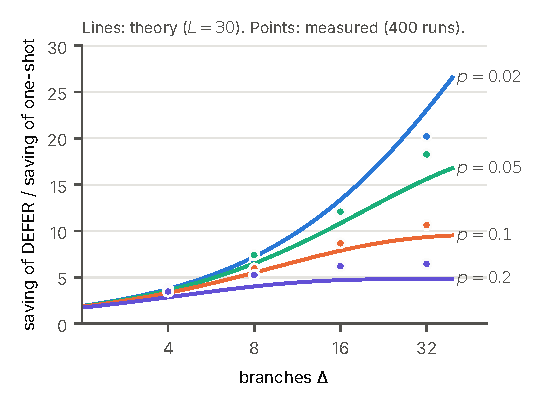
\includegraphics[width=0.62\textwidth]{figures/fig_adaptivity_gap.pdf}
\caption{Saving of DEFER relative to the best one-shot choice on the star-of-paths family ($L=30$, budget $1$), as the number of gateways $\Delta$ grows. Lines: $\frac{L}{L+1}\cdot\frac{1-(1-p)^\Delta}{p}$, the ratio of Theorem~\ref{thm:adaptivity-gap}. Points: ratios measured in simulation with 400 realizations per point; they fluctuate around the lines, most visibly at small $p$ where few realizations reach a gateway.}\label{fig:gap-curve}
\end{figure}

\begin{theorem}[Complexity of DEFER]\label{thm:defer-complexity}
Let $n_t,m_t$ be the number of vertices and edges reachable from $F_t$ in
the union of the $\theta$ samples, $r$ the number of rounds, and $\alpha$
the inverse Ackermann function. With the dominator planner, round $t$ costs
$O(\theta\,m_t\,\alpha(m_t,n_t))$ for the dominator trees plus
$O(b_t\,\theta'\,m_t\,\alpha)$ for the greedy picks ($\theta'\le\theta$);
the total is $O\bigl(\sum_t(1+b_t)\,\theta\,m_t\,\alpha\bigr)$, which is
$O(r\,b\,\theta\,m\,\alpha(m,n))$ in the worst case.
\end{theorem}

We additionally construct \emph{isocut}, a one-shot planner of our own
that adds one further kind of candidate move to AG's planner --
isolating a whole seed's out-neighborhood at once, rather than blocking
one vertex at a time -- and prove it admits a worst-case separation
(Theorem~\ref{thm:isocut-separation}, the Appendix) from AdvancedGreedy. \emph{isocut} is not itself a competing baseline from the
literature; it is reported only as an ablation, in
Appendix~\ref{sec:isocut-practice}, because it is rarely selected
on the empirical networks used there.

\emph{Intuition.} Greedy planners add one vertex at a time and credit each
with its marginal saving; when the benefit only appears after several
blocks are made together, as when isolating all out-neighbors of a seed, each
single block looks worthless and greedy never finds it.

\begin{theorem}[Isolation-move separation]\label{thm:isocut-separation}
There is a family of instances (with $2\le c\le b$ below) on which AdvancedGreedy saves $O(b)$ vertices with budget $b$,
while a planner with frontier-isolation moves saves $\Omega(N)$ for
arbitrary $N$. The statement is for AdvancedGreedy, which selects vertices one at a time by marginal single-vertex saving; we do not analyze GreedyReplace or the Sandwich greedy on this family.
\end{theorem}

\section{Experiments}\label{sec:experiments}

The experiments are designed to answer the practical questions of Table~\ref{tab:summary}: how large the benefit of adapting is on the family where the theory says it is largest (Section~\ref{sec:exp-sop}); in which regimes it appears on other graphs (Section~\ref{sec:exp-regime}); and how it compares on empirical networks (Section~\ref{sec:defer-experiments}) and with exact integer-programming baselines (Section~\ref{sec:exp-ilp}). In every comparison all policies run on the \emph{same} live-edge realization, so differences between two policies are paired. A difference is called significant when the mean paired difference in final spread exceeds twice its standard error; this is a screening rule, not a corrected test, and with many cells a few false positives are expected.
\subsection{Star-of-paths instances}\label{sec:exp-sop}

The star-of-paths family of Theorem~\ref{thm:adaptivity-gap} is the structure
for which the theory predicts an advantage of deferral: seed $s$ has $\Delta$
gateways, each active with probability $p$ and heading a private deterministic
path of $L=30$ vertices. We ran every policy of this section on identical
realizations for $\Delta\in\{4,8,16\}$, $p\in\{0.05,0.1,0.2\}$, budgets
$b\in\{1,2\}$, with 100, 50 and 20 realizations for $\Delta=4,8,16$ respectively
(fewer for the larger stars, where the ILP solves dominate the running time).
AG, GR and the ILP planners see the same sample budget as elsewhere
($\theta=100$ for greedy planners, $48$ scenarios for the ILP). This is a
constructed family, so the table shows that the predicted effect is realized
by the algorithm, not how often such structure occurs in real networks.

Figure~\ref{fig:sop} and Table~\ref{tab:sop} give the saved fraction. DEFER saves between $0.36$ and
$0.97$ of the unprotected spread. In every cell it exceeds the best of AG, GR,
COMMIT and ILP-1 by at least $0.27$ (those policies reach at most $0.48$,
$0.48$, $0.55$ and $0.64$ respectively, each in a different cell), and the paired difference in
final spread between each of AG, COMMIT and ILP-1 and DEFER has a
ratio to its standard error of at least $3.2$ in all 18 cells (54 comparisons; DEFER
is never significantly worse). DEFER-nopush equals AG exactly in every
cell: here the planned gateway is exposed in round $0$ and is committed at once
without the push-down rule, so the entire advantage comes from push-down
deferring the gateway (Lemma~\ref{lem:pushdown}), as in the worked example of
Section~\ref{sec:defer-example}. The rolling staged ILP (ILP-S)
also exploits waiting and is the best policy other than DEFER-based ones in all 18 cells;
it matches DEFER (within $0.005$ of saved fraction) in 7 cells and is below it in 11,
and is above it in 0. DEFER-ILP matches DEFER within $0.005$ in all 18 cells.

\begin{figure}[t]
\centering
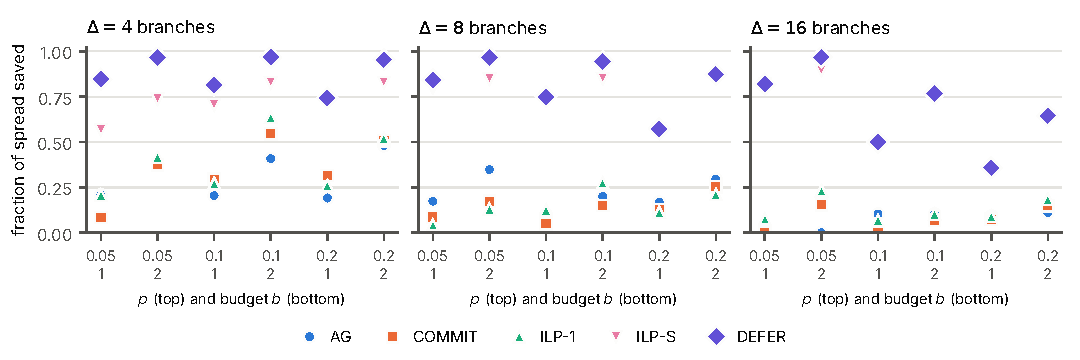
\includegraphics[width=\textwidth]{figures/fig_sop.pdf}
\caption{Fraction of spread saved on star-of-paths instances ($L=30$) by policy. Each marker is one setting: edge probability $p$ of a gateway (upper axis row) and budget $b$ (lower axis row), with 100, 50 and 20 realizations for $\Delta=4,8,16$. DEFER (large diamonds) is above every other policy in all 18 settings; Table~\ref{tab:sop} gives the numbers.}\label{fig:sop}
\end{figure}

\begin{table}[h]
\centering
\caption{Star-of-paths benchmark ($L=30$): saved fraction of spread by policy; bold is DEFER.\label{tab:sop}}
\footnotesize
\begin{tabular}{rrrrrrrrrrrr}
\hline
$\Delta$ & $p$ & $b$ & $n$ & unprot. & AG & COMMIT & ILP-1 & ILP-S & nopush & DEFER & DEFER-ILP \\
\hline
4 & 0.05 & 1 & 100 & 7.4 & 0.208 & 0.083 & 0.208 & 0.566 & 0.208 & \textbf{0.847} & 0.847 \\
4 & 0.05 & 2 & 100 & 7.4 & 0.375 & 0.375 & 0.417 & 0.737 & 0.375 & \textbf{0.968} & 0.968 \\
4 & 0.1 & 1 & 100 & 13.6 & 0.205 & 0.295 & 0.273 & 0.705 & 0.205 & \textbf{0.814} & 0.814 \\
4 & 0.1 & 2 & 100 & 13.6 & 0.409 & 0.545 & 0.636 & 0.826 & 0.409 & \textbf{0.968} & 0.968 \\
4 & 0.2 & 1 & 100 & 22.6 & 0.192 & 0.315 & 0.260 & 0.729 & 0.192 & \textbf{0.742} & 0.742 \\
4 & 0.2 & 2 & 100 & 22.6 & 0.479 & 0.507 & 0.521 & 0.828 & 0.479 & \textbf{0.954} & 0.954 \\
8 & 0.05 & 1 & 50 & 14.3 & 0.174 & 0.087 & 0.043 & 0.799 & 0.174 & \textbf{0.843} & 0.842 \\
8 & 0.05 & 2 & 50 & 14.3 & 0.348 & 0.174 & 0.130 & 0.847 & 0.348 & \textbf{0.968} & 0.968 \\
8 & 0.1 & 1 & 50 & 24.8 & 0.100 & 0.050 & 0.125 & 0.750 & 0.100 & \textbf{0.750} & 0.750 \\
8 & 0.1 & 2 & 50 & 24.8 & 0.200 & 0.150 & 0.275 & 0.848 & 0.200 & \textbf{0.944} & 0.944 \\
8 & 0.2 & 1 & 50 & 44.0 & 0.169 & 0.127 & 0.113 & 0.572 & 0.169 & \textbf{0.572} & 0.572 \\
8 & 0.2 & 2 & 50 & 44.0 & 0.296 & 0.254 & 0.211 & 0.859 & 0.296 & \textbf{0.872} & 0.872 \\
16 & 0.05 & 1 & 20 & 20.1 & 0.000 & 0.000 & 0.077 & 0.819 & 0.000 & \textbf{0.819} & 0.819 \\
16 & 0.05 & 2 & 20 & 20.1 & 0.000 & 0.154 & 0.231 & 0.893 & 0.000 & \textbf{0.968} & 0.968 \\
16 & 0.1 & 1 & 20 & 45.0 & 0.103 & 0.000 & 0.069 & 0.501 & 0.103 & \textbf{0.501} & 0.501 \\
16 & 0.1 & 2 & 20 & 45.0 & 0.103 & 0.069 & 0.103 & 0.768 & 0.103 & \textbf{0.768} & 0.768 \\
16 & 0.2 & 1 & 20 & 83.7 & 0.093 & 0.074 & 0.092 & 0.358 & 0.093 & \textbf{0.358} & 0.358 \\
16 & 0.2 & 2 & 20 & 83.7 & 0.111 & 0.148 & 0.185 & 0.645 & 0.111 & \textbf{0.645} & 0.645 \\
\hline
\end{tabular}
\end{table}

\subsection{Where does deferral help? A scan of regimes}\label{sec:exp-regime}

The small-instance benchmark of Section~\ref{sec:exp-ilp} has mostly
saturated or low-spread cells, where there is little for deferral to gain. To
see where DEFER's advantage appears, we scanned a grid of 5 graph families
(1000-node random tree, 1024-node grid, random geometric graph with mean
degree 4, Watts--Strogatz $k=4$, $\beta=0.05$, and Barab\'asi--Albert $m=2$),
3 constant edge probabilities each, and budgets $b\in\{5,20,50\}$, with 10
random seed sets of size 10 and 10 realizations per seed set (100 paired
episodes per cell). The probabilities were chosen to span sub- to near-critical
spread for each family after seeing the earlier small-instance results, so the
grid is exploratory; every cell is reported. Cells are compared pairwise on
identical realizations; the entry is the mean number of nodes by which the
spread of the other policy exceeds DEFER's (positive favors DEFER), with the
standard error of the paired difference in parentheses, in bold when the ratio
exceeds $2$. With 45 cells per comparison, about two ratios beyond $\pm2$ are
expected by chance alone.

Figure~\ref{fig:regime-heat} shows the improvement of DEFER over AG in every setting, and Figure~\ref{fig:regime-scatter} plots it against the unprotected spread per unit of budget. Against AG, DEFER is significantly better in 9 cells and significantly
worse in 0, and against COMMIT it is significantly better in 6 cells and worse in
0. The significant cells are concentrated where cascades are large:
the grid at $p=0.5$ (budgets $5,20,50$; unprotected spread about $616$ nodes;
DEFER saves $0.447$ of spread at $b=20$ against $0.335$ for AG and $0.355$ for
COMMIT), Watts--Strogatz at $p=0.5$, and random geometric graphs at moderate
$p$. Where spread is small or the budget covers the whole cascade (many cells
with $b=50$) all policies tie, and on Barab\'asi--Albert graphs there is no
significant difference anywhere.

\begin{figure}[t]
\centering
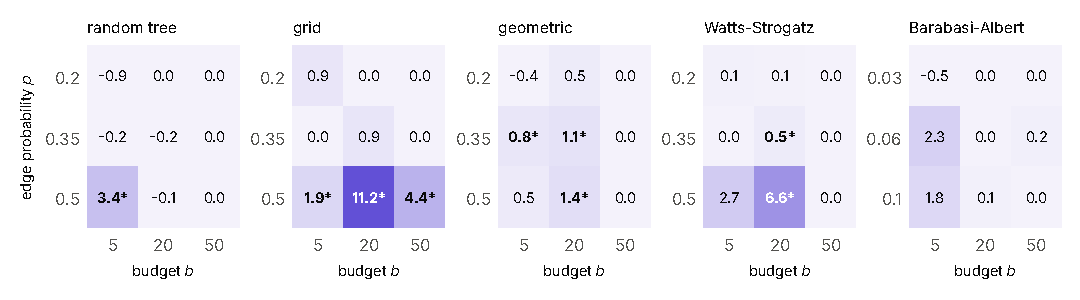
\includegraphics[width=\textwidth]{figures/fig_regime_heatmap.pdf}
\caption{Improvement of DEFER over AG, in points of the unprotected spread, for five graph families, three edge probabilities and three budgets (100 paired episodes per cell). Darker cells are larger gains; an asterisk marks a difference larger than twice its standard error; negative values appear in the lightest cells.}\label{fig:regime-heat}
\end{figure}

\begin{figure}[t]
\centering
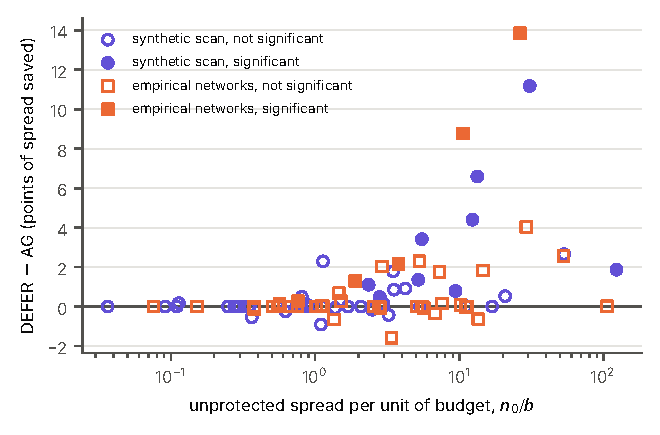
\includegraphics[width=0.66\textwidth]{figures/fig_regime_scatter.pdf}
\caption{Improvement of DEFER over AG against the unprotected spread per unit of budget, $n_0/b$, for the 45 synthetic settings and the 40 empirical-network settings; filled markers are significant (more than twice the standard error). The ratio does not separate the two groups: 12 of the 44 settings with $n_0/b\ge2$ are significant, and one significant setting has a ratio below $1$.}\label{fig:regime-scatter}
\end{figure}

\begin{table}[h]
\centering
\caption{Regime scan. Saved fraction of spread for AG and DEFER, and paired mean
differences in final spread (nodes) of AG and COMMIT relative to DEFER, with
standard errors in parentheses; positive values favor DEFER, bold marks ratio
$>2$.\label{tab:regime}}
\footnotesize
\begin{tabular}{lrrrrrrr}
\hline
Network & $p$ & $b$ & unprot. & AG & DEFER & AG$-$DEFER & COMMIT$-$DEFER \\
\hline
tree-1000 & 0.2 & 5 & 5.5 & 0.295 & 0.286 & -0.05\,(0.05) & -0.23\,(0.15) \\
tree-1000 & 0.2 & 20 & 5.5 & 0.947 & 0.947 & +0.00\,(0.00) & -0.04\,(0.08) \\
tree-1000 & 0.2 & 50 & 5.5 & 1.000 & 1.000 & +0.00\,(0.00) & +0.00\,(0.00) \\
tree-1000 & 0.35 & 5 & 12.4 & 0.375 & 0.373 & -0.02\,(0.09) & -0.07\,(0.22) \\
tree-1000 & 0.35 & 20 & 12.4 & 0.966 & 0.964 & -0.03\,(0.02) & +0.00\,(0.04) \\
tree-1000 & 0.35 & 50 & 12.4 & 1.000 & 1.000 & +0.00\,(0.00) & +0.00\,(0.00) \\
tree-1000 & 0.5 & 5 & 27.5 & 0.419 & 0.453 & \textbf{+0.94\,(0.39)} & \textbf{+1.15\,(0.50)} \\
tree-1000 & 0.5 & 20 & 27.5 & 0.979 & 0.978 & -0.02\,(0.01) & +0.04\,(0.04) \\
tree-1000 & 0.5 & 50 & 27.5 & 1.000 & 1.000 & +0.00\,(0.00) & +0.00\,(0.00) \\
grid-1024 & 0.2 & 5 & 17.6 & 0.140 & 0.148 & +0.15\,(0.11) & -0.61\,(0.47) \\
grid-1024 & 0.2 & 20 & 17.6 & 0.562 & 0.562 & +0.00\,(0.00) & +0.05\,(0.54) \\
grid-1024 & 0.2 & 50 & 17.6 & 1.000 & 1.000 & +0.00\,(0.00) & +0.00\,(0.00) \\
grid-1024 & 0.35 & 5 & 84.5 & 0.176 & 0.176 & +0.00\,(0.00) & +3.17\,(1.71) \\
grid-1024 & 0.35 & 20 & 84.5 & 0.628 & 0.637 & +0.77\,(0.49) & +0.45\,(2.01) \\
grid-1024 & 0.35 & 50 & 84.5 & 1.000 & 1.000 & +0.00\,(0.00) & +0.00\,(0.00) \\
grid-1024 & 0.5 & 5 & 615.8 & 0.064 & 0.082 & \textbf{+11.50\,(3.62)} & \textbf{+19.63\,(7.70)} \\
grid-1024 & 0.5 & 20 & 615.8 & 0.335 & 0.447 & \textbf{+68.86\,(15.08)} & \textbf{+56.62\,(17.53)} \\
grid-1024 & 0.5 & 50 & 615.8 & 0.952 & 0.996 & \textbf{+27.11\,(6.70)} & \textbf{+44.18\,(9.72)} \\
rgg-1000 & 0.2 & 5 & 16.2 & 0.235 & 0.230 & -0.07\,(0.06) & -0.44\,(0.35) \\
rgg-1000 & 0.2 & 20 & 16.2 & 0.707 & 0.712 & +0.08\,(0.12) & +0.39\,(0.31) \\
rgg-1000 & 0.2 & 50 & 16.2 & 1.000 & 1.000 & +0.00\,(0.00) & +0.00\,(0.00) \\
rgg-1000 & 0.35 & 5 & 47.0 & 0.287 & 0.294 & \textbf{+0.37\,(0.15)} & +0.12\,(0.65) \\
rgg-1000 & 0.35 & 20 & 47.0 & 0.773 & 0.784 & \textbf{+0.52\,(0.24)} & -0.26\,(0.48) \\
rgg-1000 & 0.35 & 50 & 47.0 & 1.000 & 1.000 & +0.00\,(0.00) & +0.00\,(0.00) \\
rgg-1000 & 0.5 & 5 & 103.9 & 0.330 & 0.336 & +0.55\,(0.35) & +1.91\,(1.20) \\
rgg-1000 & 0.5 & 20 & 103.9 & 0.814 & 0.828 & \textbf{+1.41\,(0.37)} & +0.40\,(0.54) \\
rgg-1000 & 0.5 & 50 & 103.9 & 1.000 & 1.000 & +0.00\,(0.00) & +0.00\,(0.02) \\
WS-1000 & 0.2 & 5 & 14.9 & 0.149 & 0.150 & +0.02\,(0.02) & +0.08\,(0.30) \\
WS-1000 & 0.2 & 20 & 14.9 & 0.591 & 0.592 & +0.01\,(0.01) & +0.21\,(0.38) \\
WS-1000 & 0.2 & 50 & 14.9 & 1.000 & 1.000 & +0.00\,(0.00) & +0.00\,(0.00) \\
WS-1000 & 0.35 & 5 & 56.2 & 0.210 & 0.210 & +0.01\,(0.01) & -0.89\,(1.07) \\
WS-1000 & 0.35 & 20 & 56.2 & 0.642 & 0.647 & \textbf{+0.27\,(0.13)} & +0.34\,(1.00) \\
WS-1000 & 0.35 & 50 & 56.2 & 1.000 & 1.000 & +0.00\,(0.00) & +0.00\,(0.00) \\
WS-1000 & 0.5 & 5 & 266.7 & 0.184 & 0.211 & +7.08\,(4.65) & +8.00\,(5.56) \\
WS-1000 & 0.5 & 20 & 266.7 & 0.673 & 0.739 & \textbf{+17.57\,(2.73)} & \textbf{+20.94\,(6.34)} \\
WS-1000 & 0.5 & 50 & 266.7 & 0.998 & 0.998 & +0.02\,(0.01) & \textbf{+0.33\,(0.10)} \\
BA-1000 & 0.03 & 5 & 1.8 & 0.286 & 0.280 & -0.01\,(0.01) & -0.04\,(0.08) \\
BA-1000 & 0.03 & 20 & 1.8 & 0.571 & 0.571 & +0.00\,(0.00) & +0.11\,(0.12) \\
BA-1000 & 0.03 & 50 & 1.8 & 0.852 & 0.852 & +0.00\,(0.00) & +0.04\,(0.06) \\
BA-1000 & 0.06 & 5 & 5.7 & 0.422 & 0.444 & +0.13\,(0.15) & +0.27\,(0.18) \\
BA-1000 & 0.06 & 20 & 5.7 & 0.661 & 0.661 & +0.00\,(0.00) & -0.01\,(0.12) \\
BA-1000 & 0.06 & 50 & 5.7 & 0.877 & 0.878 & +0.01\,(0.01) & -0.05\,(0.10) \\
BA-1000 & 0.1 & 5 & 17.4 & 0.584 & 0.602 & +0.31\,(0.23) & +0.30\,(0.33) \\
BA-1000 & 0.1 & 20 & 17.4 & 0.778 & 0.780 & +0.02\,(0.04) & +0.08\,(0.18) \\
BA-1000 & 0.1 & 50 & 17.4 & 0.937 & 0.937 & +0.00\,(0.00) & -0.01\,(0.09) \\
\hline
\end{tabular}
\end{table}

\subsection{Empirical and synthetic networks}\label{sec:defer-experiments}

To keep clear which methods are prior published work that DEFER is
compared \emph{against}, and which are our own constructions used to
isolate \emph{why} DEFER behaves as it does, we list the two groups
separately. Everything with ``DEFER'' or ``defer'' in its name below
belongs to the second group: it is a variant or ablation of our own
method, not a competing baseline.

\noindent\textbf{External one-shot baselines (prior work):}

\begin{enumerate}
\item \textbf{AdvancedGreedy (AG)} \citep{xie2023,xie2024}: picks vertices
  greedily by dominator-tree subtree size on Monte-Carlo live-edge
  samples, recomputing after each pick; the one-shot planner DEFER wraps
  by default.
\item \textbf{GreedyReplace (GR)} \citep{xie2023,xie2024}: AG followed by a
  replacement pass that swaps any picked vertex for a better one if doing
  so improves the sampled objective; the alternate planner DEFER can wrap
  (Section~\ref{sec:defer-algo}).
\item \textbf{Sandwich lower bound (LSBM)} \citep{wang2024sandwich}: a
  greedy maximum-coverage heuristic over dominator chains that gives a
  provable lower bound on the optimal one-shot solution.
\item \textbf{Proximity}: a simple one-shot heuristic that blocks the
  vertices closest to the seed set by hop distance; included as a
  na\"ive reference point, not a state-of-the-art baseline.
\end{enumerate}

\noindent\textbf{Our own ablations (all wrap or extend AG, not external
methods):}

\begin{enumerate}
\item \textbf{DEFER}: the contribution of this paper (Section~\ref{sec:defer-algo}),
  wrapping AG by default.
\item \textbf{DEFER-nopush}: DEFER with the push-down step
  (lines~\ref{alg:pushdown-start}--\ref{alg:pushdown-end} of
  Algorithm~\ref{alg:defer}) removed, so every exposed planned vertex is
  committed immediately; this is the variant Theorem~\ref{thm:defer-dominates}
  actually guarantees (Remark~\ref{rem:pushdown-counterexample}), reported
  alongside full DEFER to show push-down's empirical effect.
\item \textbf{COMMIT}: DEFER's loop with deferral itself removed --
  committing the entire plan immediately every round instead of only the
  exposed, push-down-cleared fraction; isolates the effect of re-planning
  alone from the effect of deferred commitment.
\item \textbf{isocut}: AG with one additional candidate move -- isolating
  a whole seed's out-neighborhood at once
  (Section~\ref{sec:complexity-comparison}, Theorem~\ref{thm:isocut-separation});
  a one-shot planner, not a DEFER variant, used only in
  Appendix~\ref{sec:isocut-practice}.
\item \textbf{DEFER-cut}: DEFER wrapping \emph{isocut} instead of plain
  AG, used only in Appendix~\ref{sec:isocut-practice} to check
  whether isocut's worst-case advantage survives once DEFER's adaptivity
  is layered on top.
\end{enumerate}

\noindent The networks are:

\begin{enumerate}
\item \textbf{ca-GrQc} and \textbf{ca-HepTh} \citep{leskovec2007}: arXiv
  co-authorship collaboration networks (General Relativity and High Energy
  Physics Theory categories respectively), $n=5241$ and $n=9875$.
\item \textbf{Power-grid} \citep{watts1998}: the topology of the Western
  US power grid, $n=4941$.
\item \textbf{BA(2000)}: a synthetic Barab\'asi--Albert preferential-attachment
  graph \citep{barabasi1999} with $n=2000$ and attachment parameter $m=2$.
\end{enumerate}

\noindent We also attempted soc-Epinions1 (a much larger trust network), which did not finish within budget and is left for future work. Each network is evaluated under constant activation probability $p=0.1$ and the weighted-cascade (WC) model, with 20 random seed sets of 20 vertices and 5 live-edge realizations per seed set, so every cell has 100 paired episodes, for budgets $b\in\{5,10,20,50,100\}$ (Appendix~\ref{ec:reproducibility}). Table~\ref{tab:defer-results} reports the saved fraction at budget $20$.

\begin{table}[h]
\centering
\caption{Fraction of no-intervention spread saved at budget $20$ (100 paired episodes per cell). Bold in the policy rows marks the best policy in each column. The last two rows give the mean paired improvement of DEFER over AG and over COMMIT, in percentage points of the unprotected spread, with standard errors in parentheses; bold when larger than twice the standard error.\label{tab:defer-results}}
\footnotesize
\resizebox{\textwidth}{!}{%
\begin{tabular}{@{}lcccccccc@{}}
\hline
\up & \multicolumn{2}{c}{ca-GrQc} & \multicolumn{2}{c}{ca-HepTh} & \multicolumn{2}{c}{power-grid} & \multicolumn{2}{c}{BA(2000)} \\
 & const & WC & const & WC & const & WC & const & WC \\
\hline
\up AG & 0.665 & 0.319 & 0.441 & 0.331 & 0.460 & 0.410 & 0.781 & 0.383 \\
GR & 0.657 & 0.316 & 0.444 & 0.331 & 0.460 & 0.410 & 0.771 & 0.367 \\
LSBM & 0.638 & \textbf{0.322} & 0.374 & \textbf{0.332} & 0.460 & \textbf{0.411} & 0.782 & \textbf{0.387} \\
Proximity & 0.566 & 0.179 & 0.545 & 0.233 & \textbf{0.513} & 0.394 & 0.776 & \textbf{0.386} \\
COMMIT & 0.653 & 0.290 & 0.484 & 0.225 & 0.462 & 0.369 & 0.776 & 0.360 \\
DEFER-nopush & 0.681 & 0.319 & 0.538 & 0.331 & 0.460 & 0.410 & 0.787 & 0.376 \\
DEFER & \textbf{0.683} & 0.319 & \textbf{0.580} & 0.330 & 0.459 & 0.410 & \textbf{0.794} & 0.367 \\
\hline
\up DEFER$-$AG (pp) & +1.8\,(1.2) & +0.0\,(0.0) & \textbf{+13.9}\,(4.7) & -0.1\,(0.1) & -0.1\,(0.1) & +0.0\,(0.0) & \textbf{+1.3}\,(0.6) & -1.6\,(1.3) \\
\down DEFER$-$COMMIT (pp) & +2.9\,(2.2) & +2.9\,(2.0) & +9.6\,(5.0) & \textbf{+10.5}\,(3.6) & -0.3\,(2.7) & \textbf{+4.0}\,(1.7) & +1.8\,(1.1) & +0.7\,(4.0) \\
\hline
\end{tabular}}
\end{table}

Over all 40 (network, model, budget) cells of Tables~\ref{tab:defer-results} and~\ref{tab:defer-allbudgets}, DEFER is significantly better than AG in 5 cells and never significantly worse. Its saved fraction is ahead of AG's in 17 cells, equal to three decimals in 16, and behind in 7, by at most 1.6 points. The gains concentrate on two networks under constant probability: on ca-HepTh DEFER saves $0.580$ of the spread at $b=20$ against AG's $0.441$ (a paired improvement of 13.9 points), and on BA(2000) the improvement at $b=20$ is 1.3 points. On ca-GrQc and power-grid at $b=20$ the differences are within noise, and under weighted cascade DEFER coincides with AG to three decimals on ca-GrQc, ca-HepTh and power-grid, because the push-down rule rarely fires when the weights are the small, degree-normalized ones. Against COMMIT, DEFER is significantly better in 11 cells and never significantly worse; COMMIT has the best saved fraction of AG, DEFER and COMMIT in 6 cells, by at most 4.4 points. Against GreedyReplace, DEFER is significantly better in 3 cells and significantly worse in 3, by at most 1.6 points. The push-down rule does not help here: DEFER-nopush is never significantly worse than DEFER, DEFER is significantly worse than it in two cells (by $0.11$ and $0.01$ points, borderline at $z\approx-2.03$), and the two differ by more than $0.005$ in saved fraction in 6 cells (largest $0.043$; Appendix Table~\ref{tab:defer-nopush-parity}). This is consistent with Remark~\ref{rem:pushdown-counterexample}: push-down is a local heuristic whose effect can be negative, and its benefit shows where the structure the theory describes is present (Section~\ref{sec:exp-sop}).

Figure~\ref{fig:defer-sweep} tracks AG, COMMIT and DEFER across the budget sweep under constant probability, and Table~\ref{tab:defer-allbudgets} gives the numbers. The advantage of DEFER over AG is not monotone in the budget: on ca-HepTh it is $0.0$, $2.6$, $13.9$, $8.7$ and $2.3$ points at $b=5,10,20,50,100$, and it vanishes when every policy saves nearly all of the spread.

\begin{figure}[h]
\centering
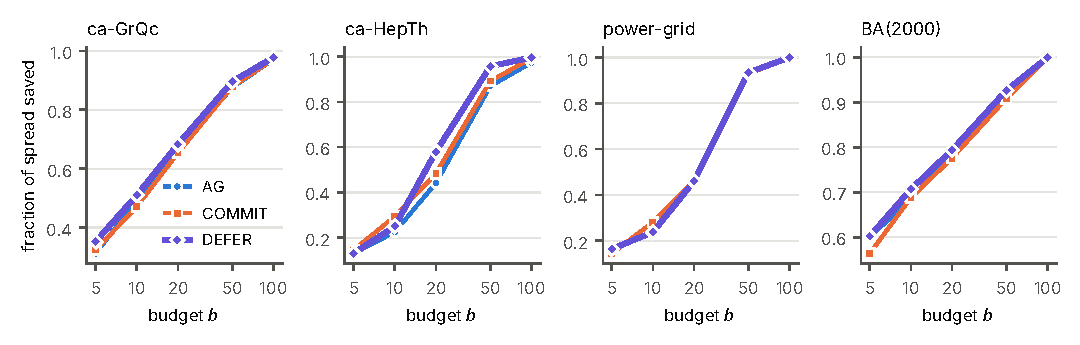
\includegraphics[width=\textwidth]{figures/defer_budget_sweep.pdf}
\caption{Fraction of no-intervention spread saved as a function of the budget, constant probability $p=0.1$, 100 paired episodes per point (Table~\ref{tab:defer-allbudgets}).\label{fig:defer-sweep}}
\end{figure}

\begin{table}[h]
\centering
\caption{Fraction of no-intervention spread saved across the budget sweep, constant probability $p=0.1$. Bold marks the best of the three policies in each cell (ties bolded on both).\label{tab:defer-allbudgets}}
\footnotesize
\resizebox{\textwidth}{!}{%
\begin{tabular}{@{}lcccccccccccc@{}}
\hline
\up & \multicolumn{3}{c}{ca-GrQc} & \multicolumn{3}{c}{ca-HepTh} & \multicolumn{3}{c}{power-grid} & \multicolumn{3}{c}{BA(2000)} \\
$b$ & AG & DEFER & COMMIT & AG & DEFER & COMMIT & AG & DEFER & COMMIT & AG & DEFER & COMMIT \\
\hline
\up 5 & 0.312 & \textbf{0.352} & 0.324 & 0.130 & 0.130 & \textbf{0.146} & 0.161 & \textbf{0.164} & 0.144 & 0.601 & \textbf{0.602} & 0.564 \\
10 & 0.492 & \textbf{0.510} & 0.471 & 0.225 & 0.251 & \textbf{0.294} & 0.237 & 0.237 & \textbf{0.280} & 0.685 & \textbf{0.707} & 0.688 \\
20 & 0.665 & \textbf{0.683} & 0.653 & 0.441 & \textbf{0.580} & 0.484 & 0.460 & 0.459 & \textbf{0.462} & 0.781 & \textbf{0.794} & 0.776 \\
50 & 0.876 & \textbf{0.896} & 0.879 & 0.870 & \textbf{0.957} & 0.892 & \textbf{0.934} & \textbf{0.934} & 0.927 & 0.924 & \textbf{0.926} & 0.908 \\
100 & 0.971 & \textbf{0.978} & 0.972 & 0.973 & \textbf{0.996} & 0.993 & \textbf{1.000} & \textbf{1.000} & \textbf{1.000} & \textbf{0.999} & \textbf{0.999} & 0.998 \\
\hline
\end{tabular}}
\end{table}

Two robustness checks are reported in Appendix~\ref{ec:seed-sensitivity}. With 50 highest-degree seeds (a more concentrated seeding), the three policies are statistically indistinguishable in 11 of 12 cells (DEFER is ahead of AG in 3, tied in 8, behind in 1), and COMMIT is significantly better than DEFER in one. The \emph{isocut} planner and DEFER-cut, two constructions of our own, give the same saved fractions as AG and DEFER to within $0.002$ (Theorem~\ref{thm:isocut-separation}'s worst-case separation does not materialize on these networks).

\subsection{Sample-average integer-programming baselines}\label{sec:exp-ilp}

\paragraph{Formulation} At a decision point the controller samples $K$
live-edge scenarios of the unobserved part of the cascade (edges out of the
frontier and out of inactive nodes; edges out of earlier active nodes have
already been tested and are dead) and solves the time-indexed sample-average
program
\[
\min \tfrac1K\sum_k\sum_v z_{kvD_k}\quad\text{s.t.}\quad
z_{kvd}\ge z_{ku,d-1}-\sum_{t<d}b_{kvt},\;\; z_{kvd}\ge z_{kv,d-1},\;\;
\sum_{v,t}b_{kvt}\le r,
\]
where $z_{kvd}$ indicates that $v$ is active by step $d$ in scenario $k$,
$b_{kvt}$ blocks $v$ before step $t$, and $r$ is the remaining budget. The
horizon $D_k$ is the unblocked cascade depth plus a slack of 4 steps, capped at
the number of reachable nodes (blocking can delay arrivals beyond the unblocked
depth, so the cap is the exact horizon and the slack is a truncation). With
the slack set to the cap, the one-shot model matches exhaustive search over all
blocking sets on the same scenarios (checked for budgets
$1$ to $3$). The models are solved with HiGHS (via SciPy) with a 30-second limit per
solve and relative gap $10^{-4}$. Two controllers use it.
ILP-1 is the one-shot optimum for the sampled scenarios, solved at time
$0$ with the whole budget (the exact counterpart of AG/GR).
ILP-S is a rolling-horizon staged model with $K=48$ scenarios in
$12$ first-step branches: blocks now are shared by all scenarios, blocks after
the first step are shared within a branch (non-anticipativity), and blocks at
step $2$ are scenario-specific recourse, which is optimistic. Only the blocks
now are committed, after which the controller observes and re-solves.

\paragraph{ILP inside DEFER} Table~\ref{tab:defer-ilp} reports the same
instances and realizations with the one-shot ILP used as DEFER's planner. The
ILP's round-0 solution is the initial plan (as for the other wrapped planners),
re-planning solves the ILP on DEFER's own samples (first 48, 10-second limit),
and plan protection and push-down are unchanged. COMMIT-ILP re-solves
every round and commits the whole plan. The solver time limit makes the
highschool2013 rows depend on machine load.

\begin{table}[h]
\centering
\caption{Saved fraction of spread with the ILP as the one-shot planner inside DEFER,
and time per episode of DEFER-ILP (seconds).\label{tab:defer-ilp}}
\footnotesize
\begin{tabular}{lrrrrrrrr}
\hline
Network & $p$ & $b$ & DEFER & ILP-1 & DEFER-ILP & nopush & COMMIT-ILP & t(DEFER-ILP)\\
\hline
dolphin & 0.1 & 2 & 0.250 & 0.319 & 0.325 & 0.319 & 0.188 & 0.04 \\
dolphin & 0.1 & 4 & 0.469 & 0.412 & 0.419 & 0.412 & 0.431 & 0.04 \\
dolphin & 0.1 & 8 & 0.744 & 0.756 & 0.762 & 0.756 & 0.706 & 0.03 \\
dolphin & 0.2 & 2 & 0.428 & 0.438 & 0.447 & 0.447 & 0.382 & 0.88 \\
dolphin & 0.2 & 4 & 0.570 & 0.570 & 0.567 & 0.572 & 0.588 & 0.78 \\
dolphin & 0.2 & 8 & 0.852 & 0.843 & 0.817 & 0.843 & 0.812 & 0.54 \\
iceland & 0.3 & 2 & 0.752 & 0.765 & 0.765 & 0.765 & 0.716 & 0.56 \\
iceland & 0.3 & 4 & 0.945 & 0.946 & 0.945 & 0.946 & 0.923 & 0.24 \\
iceland & 0.3 & 8 & 0.976 & 0.976 & 0.973 & 0.976 & 0.955 & 0.18 \\
karate & 0.2 & 2 & 0.602 & 0.590 & 0.596 & 0.596 & 0.607 & 0.11 \\
karate & 0.2 & 4 & 0.802 & 0.805 & 0.791 & 0.811 & 0.833 & 0.09 \\
workplace & 0.05 & 2 & 0.268 & 0.256 & 0.256 & 0.256 & 0.275 & 0.30 \\
workplace & 0.05 & 4 & 0.428 & 0.398 & 0.409 & 0.400 & 0.480 & 0.31 \\
workplace & 0.05 & 8 & 0.524 & 0.526 & 0.553 & 0.526 & 0.579 & 0.32 \\
BA-150 & 0.1 & 2 & 0.456 & 0.412 & 0.412 & 0.412 & 0.485 & 0.04 \\
BA-150 & 0.1 & 4 & 0.574 & 0.574 & 0.574 & 0.574 & 0.662 & 0.04 \\
BA-150 & 0.1 & 8 & 0.757 & 0.772 & 0.757 & 0.772 & 0.750 & 0.03 \\
highschool2013 & 0.03 & 4 & 0.214 & 0.181 & 0.149 & 0.149 & 0.172 & 25.36 \\
highschool2013 & 0.03 & 8 & 0.440 & 0.359 & 0.397 & 0.355 & 0.326 & 27.64 \\
\hline
\end{tabular}
\end{table}

\paragraph{Results} Figure~\ref{fig:ilp} and Table~\ref{tab:ilp} give the saved fraction of spread on
the same realizations used for every other policy (10 seed sets $\times$ 5
realizations per cell). Differences among AG, DEFER, COMMIT and ILP-1 are mostly within $0.03$
of saved fraction, while ILP-S is often far below them, and standard errors of the underlying spreads are large
relative to them (for example, $4.9$--$7.0$ on highschool2013); we did not run
paired significance tests. Counting cells where saved fractions differ by more than $0.02$:
ILP-1 is above AG in 1 of 19 cells and below it in 5; ILP-S
is above DEFER in 3 of 19 and below in 12; COMMIT is above DEFER in 11
and below in 2. On highschool2013, 47 of 100 ILP-1 solves and 26 of 971
ILP-S solves reached the time limit and returned the incumbent, and
the ILP controllers are well below the greedy ones (budget $8$: $0.312$ and
$0.162$ against $0.425$ for AG). The ILP controllers also cost orders of
magnitude more time per episode.

\begin{figure}[t]
\centering
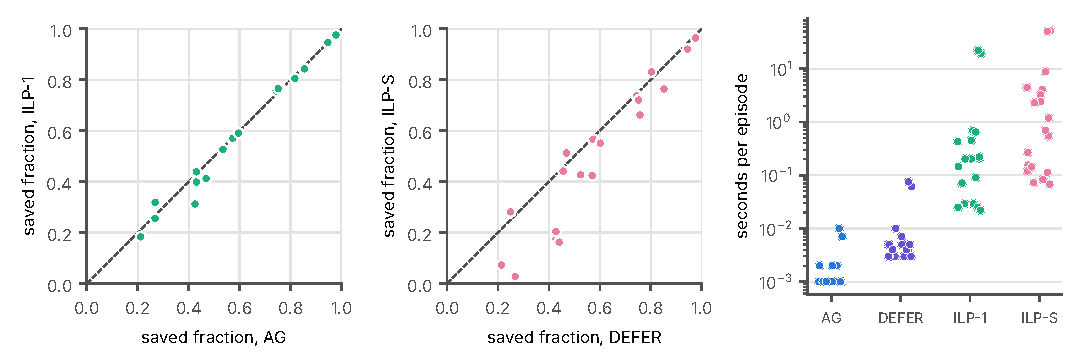
\includegraphics[width=\textwidth]{figures/fig_ilp.pdf}
\caption{Integer-programming baselines in the 19 settings of this section. Left and middle: saved fraction of the one-shot ILP against AG, and of the staged ILP against DEFER; points below the dashed diagonal mean the ILP saved less. Right: wall-clock time per episode on a logarithmic scale.}\label{fig:ilp}
\end{figure}

\begin{table}[h]
\centering
\caption{Saved fraction of spread and time per episode (seconds): greedy and DEFER
policies against the scenario-based ILP controllers. Constant edge probability
$p$; same realizations for all policies.\label{tab:ilp}}
\footnotesize
\begin{tabular}{lrrrrrrrrrr}
\hline
Network & $p$ & $b$ & AG & DEFER & COMMIT & ILP-1 & ILP-S & t(AG) & t(ILP-1) & t(ILP-S)\\
\hline
dolphin & 0.1 & 2 & 0.269 & 0.250 & 0.344 & 0.319 & 0.281 & 0.00 & 0.03 & 0.12 \\
dolphin & 0.1 & 4 & 0.469 & 0.469 & 0.500 & 0.412 & 0.512 & 0.00 & 0.03 & 0.11 \\
dolphin & 0.1 & 8 & 0.744 & 0.744 & 0.781 & 0.756 & 0.738 & 0.00 & 0.02 & 0.07 \\
dolphin & 0.2 & 2 & 0.430 & 0.428 & 0.427 & 0.438 & 0.175 & 0.00 & 0.69 & 4.03 \\
dolphin & 0.2 & 4 & 0.573 & 0.570 & 0.617 & 0.570 & 0.423 & 0.00 & 0.65 & 8.76 \\
dolphin & 0.2 & 8 & 0.855 & 0.852 & 0.820 & 0.843 & 0.763 & 0.00 & 0.45 & 3.24 \\
iceland & 0.3 & 2 & 0.752 & 0.752 & 0.809 & 0.765 & 0.720 & 0.00 & 0.43 & 4.43 \\
iceland & 0.3 & 4 & 0.946 & 0.945 & 0.938 & 0.946 & 0.920 & 0.00 & 0.20 & 0.55 \\
iceland & 0.3 & 8 & 0.978 & 0.976 & 0.974 & 0.976 & 0.964 & 0.00 & 0.14 & 0.27 \\
karate & 0.2 & 2 & 0.596 & 0.602 & 0.599 & 0.590 & 0.551 & 0.00 & 0.09 & 0.70 \\
karate & 0.2 & 4 & 0.816 & 0.802 & 0.833 & 0.805 & 0.831 & 0.00 & 0.07 & 0.14 \\
workplace & 0.05 & 2 & 0.268 & 0.268 & 0.321 & 0.256 & 0.027 & 0.00 & 0.22 & 1.19 \\
workplace & 0.05 & 4 & 0.430 & 0.428 & 0.434 & 0.398 & 0.203 & 0.00 & 0.20 & 2.41 \\
workplace & 0.05 & 8 & 0.535 & 0.524 & 0.577 & 0.526 & 0.428 & 0.00 & 0.20 & 2.29 \\
BA-150 & 0.1 & 2 & 0.471 & 0.456 & 0.507 & 0.412 & 0.441 & 0.00 & 0.03 & 0.08 \\
BA-150 & 0.1 & 4 & 0.566 & 0.574 & 0.632 & 0.574 & 0.566 & 0.00 & 0.03 & 0.07 \\
BA-150 & 0.1 & 8 & 0.757 & 0.757 & 0.721 & 0.772 & 0.662 & 0.00 & 0.03 & 0.15 \\
highschool2013 & 0.03 & 4 & 0.212 & 0.214 & 0.264 & 0.183 & 0.072 & 0.01 & 19.36 & 52.03 \\
highschool2013 & 0.03 & 8 & 0.425 & 0.440 & 0.434 & 0.312 & 0.162 & 0.01 & 21.96 & 50.35 \\
\hline
\end{tabular}
\end{table}


\subsection{Computational cost}\label{sec:complexity-comparison}

Theorem~\ref{thm:defer-complexity} states DEFER's cost as AdvancedGreedy's per-round cost multiplied by the number of rounds $r$: adaptivity is not free computationally, even though pure deferral is free in expected spread (Theorem~\ref{thm:defer-dominates}). Measured wall-clock time per episode (Appendix Table~\ref{tab:timing}) confirms the shape: AG is cheapest on every network, GR is a small constant factor above it (about $1.0$--$1.2\times$), and DEFER and COMMIT are several times above both; DEFER/AG ranges from $2.1\times$ on ca-GrQc to $4.9\times$ on ca-HepTh. COMMIT, not DEFER, is the most expensive throughout: its worse plan quality leaves the cascade active longer and adds re-planning rounds (Appendix~\ref{sec:complexity-practice}). The ILP controllers cost orders of magnitude more per episode (Section~\ref{sec:exp-ilp}).

\section{Discussion and Limitations}\label{sec:discussion}
\subsection{When does DEFER help in practice, and when is it unnecessary?}

Theorem~\ref{thm:adaptivity-gap} and Section~\ref{sec:defer-example} locate the source of DEFER's advantage: it is large when a vertex's protection is cheap to buy \emph{after} it is known to be threatened but expensive \emph{unconditionally}, that is, when activation probabilities are low relative to the branching factor and the threat, if it materializes, is large. On the star-of-paths family, where this holds by construction, the whole advantage comes from the push-down rule, since DEFER-nopush equals AG there (Section~\ref{sec:exp-sop}). Elsewhere the evidence is mixed. In the regime scan the gains appear where cascades are large (Section~\ref{sec:exp-regime}); on four empirical and synthetic networks DEFER is significantly better than AG in 5 of 40 settings, never significantly worse, and typically within a point of AG, at $2$--$5\times$ AG's compute (Table~\ref{tab:timing}); on small networks re-planning with immediate commitment is often as good (Section~\ref{sec:exp-ilp}). A practitioner should therefore ask whether the intervention has the described shape, occasional high-fan-out gatekeepers that are individually unlikely but consequential, before paying for adaptivity, and should not treat it as free and always better. DEFER-nopush is never worse than its planner up to the residual error of Remark~\ref{rem:winners-curse} (Theorem~\ref{thm:defer-dominates}); full DEFER is not (Remark~\ref{rem:pushdown-counterexample}), and the empirical differences between the two are small outside the star-of-paths family (Appendix Table~\ref{tab:defer-nopush-parity}). DEFER also assumes full-adoption feedback with negligible latency: the controller must observe each round's activations before the next round's propagation, which is realistic when suspensions or quarantines are fast relative to the cascade's own timescale, but not otherwise; noisy, delayed or partially observed feedback is open.

\subsection{Relation to exact scenario-based methods}\label{sec:discussion-exact}

Exact optimization methods for blocking, such as the Benders and bilevel
algorithms of \citet{taninmis2022,taninmis2024}, suggest a natural dynamic
baseline: a time-indexed sample-average integer program in which blocking
variables carry a time index so the budget can be spent at different steps
(Section~\ref{sec:exp-ilp}). We implemented this model directly with an
off-the-shelf solver rather than their decomposition algorithms, in a one-shot
form (ILP-1) and a rolling-horizon staged form (ILP-S),
and ran both on six networks of 34 to 327 nodes with 2--3 seeds and budgets of
2--8. Three observations follow, each limited to these small instances.

First, solving the sampled problem exactly did not beat greedy selection in
this benchmark. ILP-1 was within $0.02$ of AG's saved fraction in 13
of 19 cells, above it in one and below it in five. The sampled optimum is itself a noisy
estimate of the true optimum, so exactness on the sample need not translate
into better out-of-sample plans. Second, the staged controller did not
outperform DEFER either: ILP-S was above DEFER in 3 cells and
below in 12. Its scenario-specific recourse lets it plan to react to futures it
cannot observe, and the tree-structured non-anticipativity we imposed covers
only the first step, so we regard it as one reasonable staged formulation, not
as the best achievable one. Third, cost: the ILP controllers needed
$0.02$--$52$ s per episode against milliseconds for AG and DEFER, and on the
327-node network they frequently hit the 30-second limit and fell well behind
the greedy methods, so these formulations did not scale to the sizes where
DEFER is used.

Two further points limit what the comparison shows. On the star-of-paths family
of Theorem~\ref{thm:adaptivity-gap} (Section~\ref{sec:exp-sop}), DEFER
saves $0.36$--$0.97$ of spread and exceeds the best of AG, GR, COMMIT and
ILP-1 in all 18 cells by at least $0.27$. A separate scan of larger
synthetic networks (Section~\ref{sec:exp-regime}) finds DEFER significantly
better than AG in 9 of 45 cells and worse in 0, with the gains in large-cascade regimes; the
small-instance cells above are mostly outside that regime. COMMIT, the
re-plan-and-commit-everything ablation, was above DEFER in 11 cells and below
in 2 in this small-instance regime, so on these instances the advantage of
deferral that Section~\ref{sec:defer-example} predicts for low-probability,
high-fan-out structure did not show up; the benchmark does not contradict
Theorem~\ref{thm:adaptivity-gap}, which is a worst-case statement, but it
does not support a practical advantage of deferral at these sizes either. We
also ran the ILP as the one-shot planner inside DEFER
(DEFER-ILP, Table~\ref{tab:defer-ilp}). Wrapping the
ILP in DEFER changed little: DEFER-ILP was within $0.02$ of
ILP-1 in 15 of 19 cells, and DEFER-ILP without push-down
within $0.02$ of DEFER-ILP in 16. It was below DEFER wrapped around AG in 5
cells and above in 2, and below COMMIT in 11 cells (above in 1). Committing the
ILP's plan every round (COMMIT-ILP) was the least stable variant,
and on highschool2013 80 of its 102 solves hit the time limit. These
comparisons share the caveats above, plus one more: a solve that hits the
wall-clock limit returns an incumbent that depends on machine load, so the
highschool2013 ILP numbers are not exactly reproducible (ILP-1 at
budget $8$ scored $0.312$ in one run and $0.359$ in the repeat). Staged exact formulations with larger scenario trees, decomposition methods, or
instances with the star-of-paths structure remain to be evaluated.

\subsection{Limitations}\label{sec:conclusion}

The evidence has four limits. First, the large synthetic scan and the empirical networks use constant or weighted-cascade edge probabilities and uniformly random or highest-degree seeds; the scan grid was chosen after seeing the small-instance results, so it is exploratory. Second, the empirical-network benchmark covers four networks of up to about 10,000 vertices with 100 paired episodes per cell, so it does not show how DEFER behaves on much larger networks; an attempt on soc-Epinions1 did not finish. Third, the star-of-paths family is constructed to have the structure the theory predicts, so it shows that the algorithm realizes the effect, not how common such structure is. Fourth, DEFER assumes full-adoption feedback with negligible latency; noisy, delayed or partially observed feedback is open. We did not implement the Benders and bilevel algorithms cited in Section~\ref{sec:related}.


\appendix
\counterwithin{table}{section}
\counterwithin{figure}{section}
\counterwithin{equation}{section}
\renewcommand{\thetable}{\Alph{section}.\arabic{table}}
\renewcommand{\thefigure}{\Alph{section}.\arabic{figure}}
\renewcommand{\theequation}{\Alph{section}.\arabic{equation}}
\section{Proofs for Section~\ref{sec:defer}}\label{ec:defer-proofs}

\begin{repeatlemma}[Lemma~\ref{lem:defer-free} (Deferral is free)]
Fix a live-edge realization, the seeds, and any set $P$ with $|P|\le b$. Let
$\pi_P$ be the policy that, in every round, blocks the not-yet-blocked
vertices of $P$ that are exposed to the current frontier. Then $\pi_P$
produces exactly the same final active set as blocking $P$ at time $0$, and
blocks at most as many vertices.
\end{repeatlemma}
\begin{proof}
On a fixed realization a vertex $v$ becomes active in the first round in
which a frontier vertex has a live edge into it, i.e.\ the round after it is
first exposed. $\pi_P$ blocks $v\in P$ in that round, before its trial, so
$v$ never activates; every vertex outside $P$ faces the same set of blocked
vertices at each of its trials under both policies, because a vertex of $P$
that is never exposed never takes part in any trial. Hence the activation
sequences coincide. Vertices of $P$ that are never exposed are never
blocked.
\end{proof}

\begin{repeattheorem}[Theorem~\ref{thm:defer-dominates} (DEFER-nopush weakly dominates its planner)]
Let $P_0$ be the plan of $\mathcal P$ at round $0$, and consider
Algorithm~\ref{alg:defer} with the push-down step removed
(DEFER-nopush: every exposed planned vertex is committed
immediately). If, in every later round, the plan-protection test only ever
replaces the leftover $L=P_{t-1}\setminus C_{t-1}$ by a new plan $P'$
whose held-out sample-average saving exceeds $L$'s by more than one
held-out standard error, then the expected final spread of
DEFER-nopush is at most that of the one-shot solution $P_0$, up to
the residual error of that one-sided test (Remark~\ref{rem:winners-curse}).
\end{repeattheorem}
\begin{proof}
By Lemma~\ref{lem:defer-free} the policy that keeps $P_0$ and commits
lazily (blocking every not-yet-blocked vertex of $P_0$ the moment it is
exposed) has the same spread as blocking $P_0$ at time $0$.
DEFER-nopush differs from it only by replacing, at each round,
the uncommitted leftover by a plan that clears the plan-protection test
for the remaining budget, and then committing \emph{every} exposed vertex
of the resulting plan immediately (no push-down deferral); the committed
prefix is otherwise identical to lazily committing whichever plan is
currently standing. If every swap were only ever made when $P'$ is truly
at least as good as $L$, induction over rounds would give the claim
exactly, since replacing a standing plan by an at-least-as-good one and
then committing lazily can only weakly improve on committing the original
lazily (again by Lemma~\ref{lem:defer-free}, applied to whichever plan is
current at each round). The test instead accepts $P'$ whenever its
held-out sample-average saving exceeds $L$'s by more than one held-out
standard error -- a one-sided test against equally-good alternatives,
using concentration of the sample average (\citealp{xie2024}, applied per
candidate plan) on data disjoint from whatever $P'$ was optimized on, so
the comparison itself is not confounded by having been optimized and
tested on the same draws. This rules out the most severe form of
optimizer's-curse bias (comparing a plan against the very data used to
select it) but not the residual chance that a $P'$ that is not truly
better than $L$ still clears the $1$-SE margin on a given round's held-out
draw; Remark~\ref{rem:winners-curse} discusses this residual, which we do
not bound here. Push-down is excluded from this argument entirely: it can
permanently forfeit protection of a deferred vertex if the budget that was
supposed to remain available for it is spent elsewhere first, which is
exactly the failure mode Remark~\ref{rem:pushdown-counterexample}
exhibits.
\end{proof}

\begin{repeatremark}[Remark~\ref{rem:winners-curse} (The 1-SE margin bounds, but does not eliminate, selection bias)]
Choosing between two noisy sample averages is a textbook source of
upward-biased apparent improvement (the ``winner's curse''): if $L$ and
$P'$ were in fact equally good, the test still swaps to $P'$ whenever its
held-out average happens to exceed $L$'s by more than one standard error,
which is not a negligible event. Requiring a fresh, held-out draw for the
comparison removes the optimistic bias of optimizing and testing on the
same data, and the $1$-standard-error margin makes an accidental swap less
likely than a bare $\arg\max$ would; neither removes the residual chance
that a truly worse plan clears the margin on a given round's held-out
draw. We do not prove a bound on the resulting regret here.
\end{repeatremark}

\begin{repeatlemma}[Lemma~\ref{lem:pushdown} (Push-down is the local myopic optimum)]
Consider an exposed planned vertex $v$ whose children (its inactive
out-neighbors) jointly protect the same set as $v$ minus $v$ itself, assume
the children are exposed only through $v$, and value a budget unit at
$\lambda$ vertices. Among the two policies ``block $v$ now'' and ``block
$v$'s children if and only if $v$ activates,'' the second has smaller
expected loss (vertices lost plus $\lambda$ times budget spent) if and only
if $q_v(c_v+1/\lambda)<1$.
\end{repeatlemma}
\begin{proof}
Blocking now costs $\lambda$ and loses nothing of $v$'s set. Waiting loses
$v$ (one vertex) and spends $c_v$ units with probability $q_v$, and nothing
otherwise, while the protected set is the same in both branches by
assumption: expected loss $q_v+\lambda q_v c_v$. Comparing $\lambda$ against
$q_v+\lambda q_v c_v$ gives the stated condition. Note that $\lambda$ is
treated as a fixed price at which a budget unit can always be redeployed;
the lemma says nothing about what happens when several vertices are
deferred under this reasoning simultaneously and the budget they were all
counting on cannot cover all of them at once
(Remark~\ref{rem:pushdown-counterexample}).
\end{proof}

\begin{repeatremark}[Remark~\ref{rem:pushdown-counterexample} (Push-down does not preserve domination)]
On the star-of-paths instance with $\Delta=2$, $p=0.4$, $L=1$, $b=1$
(Section~\ref{sec:defer-example}, Remark~\ref{rem:pushdown-counterexample}
give the setup and the headline numbers, $0.96$ vs.\ $0.8$), the
case-by-case detail behind that expected spread is: with
$k\sim\mathrm{Binomial}(2,p)$ gateways active, $k\le1$ contributes spread
$k$ (the one active branch, if any, is sealed at the cost of the vertex
already reached), while $k=2$ (probability $p^2=0.16$) leaves only one
budget unit for two simultaneously-deferred children, so one branch's
path vertex activates unblocked, contributing spread $2+L=3$. Summing,
$\Pr[k{=}0]\cdot0+\Pr[k{=}1]\cdot1+\Pr[k{=}2]\cdot3=0.36(0)+0.48(1)+0.16(3)=0.96$.
\end{repeatremark}

\begin{repeattheorem}[Theorem~\ref{thm:adaptivity-gap} (The adaptivity gap of IMIN is unbounded)]
For every $\Delta\ge 2$, $p\in(0,1)$, and path length $L\ge1$ there is an
instance with maximum out-degree $\Delta$, budget $1$, on which the best
one-shot solution and DEFER have expected savings $p(L+1)$ and
$L(1-(1-p)^\Delta)$ respectively, so DEFER's saving is
$\frac{L}{L+1}\cdot\frac{1-(1-p)^\Delta}{p}$ times the one-shot saving, a
factor tending to $(1-(1-p)^\Delta)/p$ (which itself tends to $\Delta$ as
$p\to0$) as $L\to\infty$; the ratio of the two policies' expected spreads
is, at every finite $L$, strictly \emph{less} than
$\frac{(\Delta-1)p}{\Delta p-1+(1-p)^\Delta}$, increasing to this value only
in the limit $L\to\infty$, which (taken before $p\to0$, for fixed $\Delta$)
diverges.
\end{repeattheorem}
\begin{proof}
Seed $s$ has out-neighbors $a_1,\dots,a_\Delta$ with $p(s,a_i)=p$; each
$a_i$ starts a private directed path of length $L$ with edge probability
$1$. Any one-shot solution with budget $1$ blocks one vertex; blocking
$a_i$ (or a vertex on its path) saves exactly $L+1$ vertices if $a_i$ is
activated, which happens with probability $p$, and nothing otherwise, so
its expected saving is $p(L+1)$ and its expected spread is
$(\Delta-1)p(L+1)$ (the other $\Delta-1$ branches are unprotected). DEFER
observes $N_1=\{a_i:(s,a_i)\text{ live}\}$ and blocks the first path vertex
of one activated branch (its plan at round $0$ is a branch head $a_i$ with
$q=p$, $c=1$, and $\lambda\approx pL$, so the push-down rule
$p(1+1/(pL))<1$ defers it); if $k$ branches are active the spread is
$(k-1)^+L+k$. Its expected saving is $L\Pr[k\ge1]=L(1-(1-p)^\Delta)$ (one
branch's continuation is sealed for the cost of the vertex already reached,
regardless of $k$) and its expected spread is
$\mathbb E[(k-1)^+]L+\Delta p=(\Delta p-1+(1-p)^\Delta)L+\Delta p$, using
$\mathbb E[(k-1)^+]=\mathbb E[k]-\Pr[k\ge1]=\Delta p-(1-(1-p)^\Delta)$.

Two distinct ratios follow from these exact expressions. The \emph{saving}
ratio is $\frac{L(1-(1-p)^\Delta)}{p(L+1)}=\frac{L}{L+1}\cdot
\frac{1-(1-p)^\Delta}{p}$, increasing in $L$ to the limit
$(1-(1-p)^\Delta)/p$, which tends to $\Delta$ as $p\to0$ (since
$1-(1-p)^\Delta=\Delta p-\binom\Delta2p^2+O(p^3)$). The \emph{spread} ratio
is $\frac{(\Delta-1)p(L+1)}{(\Delta p-1+(1-p)^\Delta)L+\Delta p}$. Writing
$A=(\Delta-1)p$, $B=\Delta p-1+(1-p)^\Delta$, $C=\Delta p$, this is
$A(L+1)/(BL+C)$, whose derivative with respect to $L$ has the sign of
$A(C-B)$; since $C-B=1-(1-p)^\Delta>0$, the ratio is strictly increasing in
$L$ for every finite $L\ge1$ and tends to its supremum $A/B=\frac{(\Delta-1)p}
{\Delta p-1+(1-p)^\Delta}$ only as $L\to\infty$ -- so at any finite $L$ the
spread ratio is strictly below this value, not at least it. Taking
$L\to\infty$ first (for fixed $\Delta,p$) and only then $p\to0$: the
denominator $B$ behaves like $\binom\Delta2p^2$ as $p\to0$ (the $O(p)$
terms cancel), so the $L\to\infty$ limit $A/B$ behaves like
$\frac{(\Delta-1)p}{\binom\Delta2p^2}=\frac{2}{\Delta p}\to\infty$ --
already unbounded at $\Delta=2$, independently of the saving ratio's
$\Delta\to\infty$ argument, but only once $L$ has been sent to infinity
first: for any \emph{fixed} $L$, the same ratio $A(L+1)/(BL+C)$ tends
instead to $A(L+1)/C=(\Delta-1)(L+1)/\Delta$ as $p\to0$ (since $B\to0$
faster than $C$), a finite constant, so the order of the two limits is not
interchangeable. The two ratios are genuinely different quantities -- the
savings' ratio bound does not apply to the spreads' ratio -- and both
statements above are established directly from the same exact closed
forms, with no approximation beyond the stated limits.
\end{proof}

\begin{repeattheorem}[Theorem~\ref{thm:defer-complexity} (Complexity of DEFER)]
Let $n_t,m_t$ be the number of vertices and edges reachable from $F_t$ in
the union of the $\theta$ samples, $r$ the number of rounds, and $\alpha$
the inverse Ackermann function. With the dominator planner, round $t$
costs $O(\theta\,m_t\,\alpha(m_t,n_t))$ for the dominator trees plus
$O(b_t\,\theta'\,m_t\,\alpha)$ for the greedy picks; the total is
$O\bigl(\sum_t(1+b_t)\,\theta\,m_t\,\alpha\bigr)$, which is
$O(r\,b\,\theta\,m\,\alpha(m,n))$ in the worst case.
\end{repeattheorem}
\begin{proof}
Each dominator tree is computed by the Cooper--Harvey--Kennedy iteration
on the reachable subgraph (near-linear; the Lengauer--Tarjan analysis gives
the $\alpha$ bound). Drawing $\theta$ live-edge samples reachable from
$F_t$ (Algorithm~\ref{alg:defer}) is a breadth-first search per sample. Recomputation after a pick is restricted to samples
whose cached reach set contains the picked vertex, which is exactly the
set of samples whose dominator tree can change. Summing over picks and
rounds gives the bound.
\end{proof}

\begin{repeattheorem}[Theorem~\ref{thm:isocut-separation} (Isolation-move separation)]
There is a family of instances (with $2\le c\le b$ below) on which AdvancedGreedy saves $O(b)$ vertices with budget $b$,
while a planner with frontier-isolation moves saves $\Omega(N)$ for
arbitrary $N$.
\end{repeattheorem}
\begin{proof}
Construction: a decoy seed with $b+1$ out-neighbors, each with one private
leaf (single-vertex saving 2); a real seed with $2\le c\le b$ out-neighbors (so that no single out-neighbor disconnects $R$), all
of which point to every vertex of a region $R$ of $N$ vertices whose
vertices have no private successors. Every single vertex in $R$ or among
the real seed's out-neighbors saves at most 1, so a rule that picks by marginal single-vertex saving, as AdvancedGreedy does,
spends the budget on decoy neighbors (saving $2b$), whereas
isolating the real seed saves $N+c$ at cost $c$.
\end{proof}

\section{Seed Selection, Cost and Isolation-Move Ablations}\label{ec:seed-sensitivity}

\subsection{Seed-selection sensitivity}

The main-body results seed with 20 uniformly random vertices. We additionally ran a sweep with 50 highest-degree seeds, a harder and more concentrated seeding, on the same networks with budgets $10,20,50$, constant probability $p=0.1$, 20 seed sets and 5 realizations per seed set (Table~\ref{tab:defer-degree-seeds}). Across the 12 cells no difference between AG and DEFER is significant (DEFER is ahead in 3, tied to three decimals in 8, behind in 1), and COMMIT is significantly better than DEFER in one cell. High-degree seeding makes the cascade large at the start and leaves little for deferral to buy.

\begin{table}[h]
\centering
\caption{Fraction of spread saved, 50 highest-degree seeds, constant probability $p=0.1$, 100 paired episodes per cell. Bold marks the best of the three policies per cell (ties bolded on both).\label{tab:defer-degree-seeds}}
\footnotesize
\resizebox{\textwidth}{!}{%
\begin{tabular}{@{}lcccccccccccc@{}}
\hline
\up & \multicolumn{3}{c}{ca-GrQc} & \multicolumn{3}{c}{ca-HepTh} & \multicolumn{3}{c}{power-grid} & \multicolumn{3}{c}{BA(2000)} \\
$b$ & AG & DEFER & COMMIT & AG & DEFER & COMMIT & AG & DEFER & COMMIT & AG & DEFER & COMMIT \\
\hline
\up 10 & 0.188 & 0.190 & \textbf{0.191} & 0.103 & 0.103 & \textbf{0.111} & 0.080 & 0.080 & \textbf{0.082} & 0.320 & 0.320 & \textbf{0.322} \\
20 & 0.306 & \textbf{0.307} & \textbf{0.307} & 0.191 & 0.191 & \textbf{0.192} & 0.124 & 0.124 & \textbf{0.130} & 0.369 & 0.370 & \textbf{0.372} \\
50 & 0.492 & 0.493 & \textbf{0.500} & \textbf{0.373} & \textbf{0.373} & 0.368 & \textbf{0.232} & \textbf{0.232} & 0.229 & \textbf{0.444} & \textbf{0.444} & \textbf{0.445} \\
\hline
\end{tabular}}
\end{table}

\subsection{Complexity in practice}\label{sec:complexity-practice}

Table~\ref{tab:timing} gives the wall-clock time per episode behind the main text's cost discussion (Section~\ref{sec:complexity-comparison}), including planning, measured by the same runs as Table~\ref{tab:defer-results}. COMMIT, despite executing the same per-round loop as DEFER, costs more than DEFER on every network: its plans are of lower quality and leave the cascade active longer, adding re-planning rounds.

\begin{table}[h]
\centering
\caption{Wall-clock time per episode (seconds), budget $20$, constant probability $p=0.1$, pure Python on one core.\label{tab:timing}}
\small
\begin{tabular}{@{}lccccc@{}}
\hline
\up network ($n$) & AG & GR & DEFER & COMMIT & DEFER/AG \\
\hline
\up ca-GrQc (5241) & 0.108 & 0.116 & 0.223 & 0.592 & 2.1$\times$ \\
ca-HepTh (9875) & 0.297 & 0.300 & 1.470 & 1.527 & 4.9$\times$ \\
power-grid (4941) & 0.005 & 0.006 & 0.012 & 0.031 & 2.4$\times$ \\
BA(2000) (2000) & 0.008 & 0.009 & 0.031 & 0.047 & 3.9$\times$ \\
\hline
\end{tabular}
\end{table}

\subsection{Isolation moves in practice}\label{sec:isocut-practice}

\emph{isocut} (AG extended with a frontier-isolation move) and DEFER-cut (DEFER wrapping \emph{isocut}) are our own constructions, not literature baselines. Theorem~\ref{thm:isocut-separation} gives a worst-case family on which isolation moves save $\Omega(N)$ against $O(b)$ for AdvancedGreedy. Table~\ref{tab:isocut} checks whether this appears on the networks used here: it does not. \emph{isocut} equals AG to three decimals on all four networks, and DEFER-cut is within $0.002$ of DEFER. Real collaboration and infrastructure networks rarely have a seed whose entire out-neighborhood points into an otherwise unreachable region, so the move is a documented worst-case possibility, not a component of the default algorithm.

\begin{table}[h]
\centering
\caption{Fraction of spread saved, isolation-move ablations, 50 highest-degree seeds, budget $20$, constant probability $p=0.1$.\label{tab:isocut}}
\small
\begin{tabular}{@{}lcccc@{}}
\hline
\up network & AG & isocut & DEFER & DEFER-cut \\
\hline
\up ca-GrQc & 0.306 & 0.306 & 0.307 & 0.309 \\
ca-HepTh & 0.191 & 0.191 & 0.191 & 0.191 \\
power-grid & 0.124 & 0.124 & 0.124 & 0.124 \\
BA(2000) & 0.369 & 0.369 & 0.370 & 0.370 \\
\hline
\end{tabular}
\end{table}

\section{Experimental Protocol}\label{ec:reproducibility}

\paragraph{Empirical networks (Section~\ref{sec:defer-experiments}).} Graphs: ca-GrQc, ca-HepTh, a power-grid network and a Barab\'asi--Albert graph with 2000 vertices. Probabilities: constant $p=0.1$ and the weighted-cascade model. Seeds: 20 uniformly random vertices per seed set (50 highest-degree vertices in the robustness run), 20 seed sets per cell. Budgets: $5,10,20,50,100$ ($10,20,50$ in the robustness run). Each seed set has 5 independent live-edge realizations, and every policy runs on the same realization with the same total budget (common random numbers), so differences are attributable to the policy alone; planners use $\theta=100$ sampled live-edge subgraphs. Policies: none; AdvancedGreedy, GreedyReplace, the Sandwich lower bound and proximity-to-seeds (one-shot); COMMIT, DEFER and DEFER-nopush, all wrapping AdvancedGreedy. Reported: final spread beyond the seeds, saved fraction (one minus total spread over total unprotected spread), paired differences with standard errors, and wall-clock time per episode including planning. A paired difference is called significant when it exceeds twice its standard error; this is a screening rule, not a corrected test, and across 40 cells a few false positives are expected.

Table~\ref{tab:defer-nopush-parity} gives the difference in saved fraction between full DEFER and DEFER-nopush.

\begin{table}[h]
\centering
\caption{Saved fraction of full DEFER minus saved fraction of DEFER-nopush, by network, model and budget.\label{tab:defer-nopush-parity}}
\footnotesize
\resizebox{\textwidth}{!}{%
\begin{tabular}{@{}lcccccccc@{}}
\hline
\up & \multicolumn{2}{c}{ca-GrQc} & \multicolumn{2}{c}{ca-HepTh} & \multicolumn{2}{c}{power-grid} & \multicolumn{2}{c}{BA(2000)} \\
$b$ & const & WC & const & WC & const & WC & const & WC \\
\hline
\up 5 & +0.014 & -0.000 & +0.000 & +0.000 & +0.003 & +0.001 & -0.000 & -0.009 \\
10 & +0.001 & -0.000 & +0.000 & +0.000 & +0.000 & +0.000 & +0.004 & -0.008 \\
20 & +0.002 & -0.000 & +0.043 & -0.000 & -0.001 & +0.000 & +0.006 & -0.009 \\
50 & +0.000 & +0.000 & +0.002 & +0.000 & +0.000 & +0.000 & -0.001 & -0.001 \\
100 & +0.001 & -0.000 & -0.000 & +0.000 & +0.000 & +0.000 & +0.000 & +0.000 \\
\hline
\end{tabular}}
\end{table}

The two differ by more than $0.005$ in 6 of 40 cells, with a largest absolute difference of $0.043$; DEFER is never significantly better than DEFER-nopush and is significantly worse in two cells by $0.11$ and $0.01$ points.

\paragraph{Other experiments} The star-of-paths, regime-scan and integer-programming experiments are described in Sections~\ref{sec:exp-sop}, \ref{sec:exp-regime} and~\ref{sec:exp-ilp}. All of them use the same design: every policy runs on the same live-edge realization, and per-instance results are part of the data described in the data availability statement.

\section*{CRediT authorship contribution statement}
\textbf{Quang-Vinh Dang:} Conceptualization, Methodology, Software, Validation, Formal analysis, Investigation, Data curation, Visualization, Writing -- original draft, Writing -- review \& editing. \textbf{Dat Le:} Writing -- review \& editing. \textbf{Minh Ngoc Dinh:} Writing -- review \& editing.

\section*{Declaration of competing interest}
The authors declare that there are no known competing financial interests or personal relationships that could have appeared to influence the work reported in this paper.

\section*{Funding}
This research did not receive any specific grant from funding agencies in the public, commercial, or not-for-profit sectors.

\section*{Data availability}
The code, scripts, networks used and per-instance results that reproduce every table and figure are available at \url{https://github.com/vinhqdang/trace_e}.

\section*{Declaration of generative AI and AI-assisted technologies in the manuscript preparation process}
During the preparation of this work the authors used Claude (Anthropic) to support the writing of the manuscript and to assist in writing and running the code, figures and diagrams. After using this tool, the authors reviewed and edited the content as needed and take full responsibility for the content of the published article.

\begin{thebibliography}{99}
\providecommand{\natexlab}[1]{#1}
\providecommand{\url}[1]{\texttt{#1}}

\bibitem[{Xie et~al.(2023)Xie, Zhang, Wang, Lin, and Zhang}]{xie2023}
Xie J, Zhang F, Wang K, Lin X, Zhang W. Minimizing the influence of misinformation via vertex blocking. In: Proceedings of the 39th IEEE International Conference on Data Engineering (ICDE); 2023, p. 3096-108. \url{https://doi.org/10.1109/ICDE55515.2023.00066}.

\bibitem[{Xie et~al.(2025)Xie, Zhang, Wang, Liu, Lin, and Zhang}]{xie2024}
Xie J, Zhang F, Wang K, Liu J, Lin X, Zhang W. Influence minimization via blocking strategies. INFORMS J Comput 2025;37(6):1587-604. \url{https://doi.org/10.1287/ijoc.2024.0591}.

\bibitem[{Kempe et~al.(2003)Kempe, Kleinberg, and Tardos}]{kempe2003}
Kempe D, Kleinberg J, Tardos É. Maximizing the spread of influence through a social network. In: Proceedings of the 9th ACM SIGKDD International Conference on Knowledge Discovery and Data Mining (KDD); 2003, p. 137-46. \url{https://doi.org/10.1145/956750.956769}.

\bibitem[{Wang et~al.(2024)Wang, Wu, Wang, Zhang, Qin, Zhang, and Lin}]{wang2024sandwich}
Wang J, Wu Y, Wang X, Zhang Y, Qin L, Zhang W, et al. Efficient influence minimization via node blocking. Proc VLDB Endow 2024;17(10):2501-13. \url{https://doi.org/10.14778/3675034.3675042}.

\bibitem[{Shi et~al.(2019)}]{shi2019}
Shi Q, Wang C, Ye D, Chen J, Feng Y, Chen C. Adaptive influence blocking: Minimizing the negative spread by observation-based policies. In: Proceedings of the 35th IEEE International Conference on Data Engineering (ICDE); 2019, p. 1502-13. \url{https://doi.org/10.1109/ICDE.2019.00135}.

\bibitem[{Leskovec et~al.(2007b)}]{leskovec2007b}
Leskovec J, Krause A, Guestrin C, Faloutsos C, VanBriesen J, Glance N. Cost-effective outbreak detection in networks. In: Proceedings of the 13th ACM SIGKDD International Conference on Knowledge Discovery and Data Mining; 2007, p. 420-9. \url{https://doi.org/10.1145/1281192.1281239}.

\bibitem[{Borgs et~al.(2014)}]{borgs2014}
Borgs C, Brautbar M, Chayes J, Lucier B. Maximizing social influence in nearly optimal time. In: Proceedings of the 25th Annual ACM-SIAM Symposium on Discrete Algorithms (SODA); 2014, p. 946-57. \url{https://doi.org/10.1137/1.9781611973402.70}.

\bibitem[{Tang et~al.(2014)}]{tang2014}
Tang Y, Xiao X, Shi Y. Influence maximization: Near-optimal time complexity meets practical efficiency. In: Proceedings of the 2014 ACM SIGMOD International Conference on Management of Data; 2014, p. 75-86. \url{https://doi.org/10.1145/2588555.2593670}.

\bibitem[{Li et~al.(2018)}]{li2018}
Li Y, Fan J, Wang Y, Tan KL. Influence maximization on social graphs: A survey. IEEE Trans Knowl Data Eng 2018;30(10):1852-72. \url{https://doi.org/10.1109/TKDE.2018.2807843}.

\bibitem[{Chen et~al.(2010)Chen, Wang, and Wang}]{chen2010}
Chen W, Wang C, Wang Y. Scalable influence maximization for prevalent viral marketing in large-scale social networks. In: Proceedings of the 16th ACM SIGKDD International Conference on Knowledge Discovery and Data Mining; 2010, p. 1029-38. \url{https://doi.org/10.1145/1835804.1835934}.

\bibitem[{Golovin and Krause(2011)}]{golovinkrause2011}
Golovin D, Krause A. Adaptive submodularity: Theory and applications in active learning and stochastic optimization. J Artif Intell Res 2011;42:427-86.

\bibitem[{Seeman and Singer(2013)}]{seemansinger2013}
Seeman L, Singer Y. Adaptive seeding in social networks. In: Proceedings of the 54th Annual IEEE Symposium on Foundations of Computer Science (FOCS); 2013, p. 459-68. \url{https://doi.org/10.1109/FOCS.2013.56}.

\bibitem[{Tong et~al.(2017)}]{tong2017}
Tong G, Wu W, Tang S, Du DZ. Adaptive influence maximization in dynamic social networks. IEEE/ACM Trans Netw 2017;25(1):112-25.

\bibitem[{Sun et~al.(2018)}]{sun2018}
Sun L, Huang W, Yu PS, Chen W. Multi-round influence maximization. In: Proceedings of the 24th ACM SIGKDD International Conference on Knowledge Discovery and Data Mining; 2018, p. 2249-58. \url{https://doi.org/10.1145/3219819.3220101}.

\bibitem[{Yuan and Tang(2017)}]{yuan2017}
Yuan J, Tang SJ. No time to observe: Adaptive influence maximization with partial feedback. In: Proceedings of the 26th International Joint Conference on Artificial Intelligence (IJCAI); 2017, p. 3908-14. \url{https://doi.org/10.24963/ijcai.2017/546}.

\bibitem[{Asadpour and Nazerzadeh(2016)}]{asadpournazerzadeh2016}
Asadpour A, Nazerzadeh H. Maximizing stochastic monotone submodular functions. Manag Sci 2016;62(8):2374-91. \url{https://doi.org/10.1287/mnsc.2015.2254}.

\bibitem[{Dean et~al.(2008)Dean, Goemans, and Vondr\'ak}]{deangoemansvondrak2008}
Dean BC, Goemans MX, Vondrák J. Approximating the stochastic knapsack problem: The benefit of adaptivity. Math Oper Res 2008;33(4):945-64. \url{https://doi.org/10.1287/moor.1080.0330}.

\bibitem[{Xiang et~al.(2024)Xiang, Wang, Wu, Wang, Chen, and Zhang}]{xiang2024}
Xiang F, Wang J, Wu Y, Wang X, Chen C, Zhang Y. Rumor blocking with pertinence set in large graphs. World Wide Web 2024;27(1):6.

\bibitem[{Kimura et~al.(2008)Kimura, Saito, and Motoda}]{kimura2008}
Kimura M, Saito K, Motoda H. Minimizing the spread of contamination by blocking links in a network. In: Proceedings of the 23rd AAAI Conference on Artificial Intelligence; 2008, p. 1175-80.

\bibitem[{Budak et~al.(2011)Budak, Agrawal, and El~Abbadi}]{budak2011}
Budak C, Agrawal D, El Abbadi A. Limiting the spread of misinformation in social networks. In: Proceedings of the 20th International Conference on World Wide Web (WWW); 2011, p. 665-74. \url{https://doi.org/10.1145/1963405.1963499}.

\bibitem[{He et~al.(2012)}]{he2012}
He X, Song G, Chen W, Jiang Q. Influence blocking maximization in social networks under the competitive linear threshold model. In: Proceedings of the 2012 SIAM International Conference on Data Mining (SDM); 2012, p. 463-74. \url{https://doi.org/10.1137/1.9781611972825.40}.

\bibitem[{Nguyen et~al.(2012)}]{nguyen2012}
Nguyen NP, Yan G, Thai MT, Eidenbenz S. Containment of misinformation spread in online social networks. In: Proceedings of the 4th Annual ACM Web Science Conference (WebSci); 2012, p. 213-22. \url{https://doi.org/10.1145/2380718.2380746}.

\bibitem[{Wang et~al.(2013)Wang, Zhao, Chen, Li, Zhang, and Xia}]{wang2013blocking}
Wang S, Zhao X, Chen Y, Li Z, Zhang K, Xia J. Negative influence minimizing by blocking nodes in social networks. In: Late-Breaking Developments in the Field of Artificial Intelligence, Papers Presented at the 27th AAAI Conference on Artificial Intelligence; 2013, p. 134-6.

\bibitem[{Yan et~al.(2020)}]{yan2020}
Yan R, Li D, Wu W, Du DZ, Wang Y. Minimizing influence of rumors by blockers on social networks: Algorithms and analysis. IEEE Trans Netw Sci Eng 2020;7(3):1067-78. \url{https://doi.org/10.1109/TNSE.2019.2903272}.

\bibitem[{Fan et~al.(2013)}]{fan2013}
Fan L, Lu Z, Wu W, Thuraisingham B, Ma H, Bi Y. Least cost rumor blocking in social networks. In: Proceedings of the 33rd IEEE International Conference on Distributed Computing Systems (ICDCS); 2013, p. 540-9. \url{https://doi.org/10.1109/ICDCS.2013.34}.

\bibitem[{Kuhlman et~al.(2013)}]{kuhlman2013}
Kuhlman CJ, Tuli G, Swarup S, Marathe MV, Ravi SS. Blocking simple and complex contagion by edge removal. In: Proceedings of the 13th IEEE International Conference on Data Mining (ICDM); 2013, p. 399-408. \url{https://doi.org/10.1109/ICDM.2013.47}.

\bibitem[{Tong et~al.(2012)}]{tong2012}
Tong H, Prakash BA, Eliassi-Rad T, Faloutsos M, Faloutsos C. Gelling, and melting, large graphs by edge manipulation. In: Proceedings of the 21st ACM International Conference on Information and Knowledge Management (CIKM); 2012, p. 245-54. \url{https://doi.org/10.1145/2396761.2396795}.

\bibitem[{Khalil et~al.(2014)}]{khalil2014}
Khalil EB, Dilkina B, Song L. Scalable diffusion-aware optimization of network topology. In: Proceedings of the 20th ACM SIGKDD International Conference on Knowledge Discovery and Data Mining; 2014, p. 1226-35. \url{https://doi.org/10.1145/2623330.2623704}.

\bibitem[{Wang et~al.(2016)}]{wang2016drimux}
Wang B, Chen G, Fu L, Song L, Wang X. DRIMUX: Dynamic rumor influence minimization with user experience in social networks. In: Proceedings of the 30th AAAI Conference on Artificial Intelligence (AAAI); 2016, p. 791-7. \url{https://doi.org/10.1609/aaai.v30i1.10063}.

\bibitem[{Tong et~al.(2018)}]{tong2018}
Tong G, Wu W, Du DZ. Distributed rumor blocking with multiple positive cascades. IEEE Trans Comput Soc Syst 2018;5(2):468-80.

\bibitem[{Farajtabar et~al.(2017)}]{farajtabar2017}
Farajtabar M, Yang J, Ye X, Xu H, Trivedi R, Khalil E, et al. Fake news mitigation via point process based intervention. In: Proceedings of the 34th International Conference on Machine Learning (ICML); 2017, p. 1097-106.

\bibitem[{Zareie and Sakellariou(2021)}]{zareie2021}
Zareie A, Sakellariou R. Minimizing the spread of misinformation in online social networks: A survey. J Netw Comput Appl 2021;186:103094. \url{https://doi.org/10.1016/j.jnca.2021.103094}.

\bibitem[{Pastor-Satorras and Vespignani(2002)}]{pastor2002}
Pastor-Satorras R, Vespignani A. Immunization of complex networks. Phys Rev E 2002;65(3):036104. \url{https://doi.org/10.1103/PhysRevE.65.036104}.

\bibitem[{Cohen et~al.(2003)Cohen, Havlin, and ben-Avraham}]{cohen2003}
Cohen R, Havlin S, ben-Avraham D. Efficient immunization strategies for computer networks and populations. Phys Rev Lett 2003;91(24):247901. \url{https://doi.org/10.1103/PhysRevLett.91.247901}.

\bibitem[{Preciado et~al.(2014)}]{preciado2014}
Preciado VM, Zargham M, Enyioha C, Jadbabaie A, Pappas GJ. Optimal resource allocation for network protection against spreading processes. IEEE Trans Control Netw Syst 2014;1(1):99-108. \url{https://doi.org/10.1109/TCNS.2014.2310911}.

\bibitem[{Li and Aprahamian(2024)}]{li2024}
Li S, Aprahamian H. Quantifying the benefits of customized vaccination strategies: A network-based optimization approach. Nav Res Logist 2024;71(1):64-86. \url{https://doi.org/10.1002/nav.22134}.

\bibitem[{Smith and Song(2020)}]{smith2020}
Smith JC, Song Y. A survey of network interdiction models and algorithms. Eur J Oper Res 2020;283(3):797-811. \url{https://doi.org/10.1016/j.ejor.2019.06.024}.

\bibitem[{Cormican et~al.(1998)Cormican, Morton, and Wood}]{cormican1998}
Cormican KJ, Morton DP, Wood RK. Stochastic network interdiction. Oper Res 1998;46(2):184-97. \url{https://doi.org/10.1287/opre.46.2.184}.

\bibitem[{Birge and Louveaux(2011)}]{birge2011}
Birge JR, Louveaux F. Introduction to Stochastic Programming. 2nd ed. New York: Springer; 2011. \url{https://doi.org/10.1007/978-1-4614-0237-4}.

\bibitem[{Kleywegt et~al.(2002)Kleywegt, Shapiro, and Homem-de-Mello}]{kleywegt2002}
Kleywegt AJ, Shapiro A, Homem-de-Mello T. The sample average approximation method for stochastic discrete optimization. SIAM J Optim 2002;12(2):479-502. \url{https://doi.org/10.1137/S1052623499363220}.

\bibitem[{Roohnavazfar et~al.(2019)Roohnavazfar, Manerba, De~Martin, and Tadei}]{roohnavazfar2019}
Roohnavazfar M, Manerba D, De Martin JC, Tadei R. Optimal paths in multi-stage stochastic decision networks. Oper Res Perspect 2019;6:100124. \url{https://doi.org/10.1016/j.orp.2019.100124}.

\bibitem[{Rempel and Cai(2021)}]{rempel2021}
Rempel M, Cai J. A review of approximate dynamic programming applications within military operations research. Oper Res Perspect 2021;8:100204. \url{https://doi.org/10.1016/j.orp.2021.100204}.

\bibitem[{Gupta et~al.(2016)Gupta, Nagarajan, and Singla}]{gupta2016}
Gupta A, Nagarajan V, Singla S. Algorithms and adaptivity gaps for stochastic probing. In: Proceedings of the 27th Annual ACM-SIAM Symposium on Discrete Algorithms (SODA); 2016, p. 1731-47. \url{https://doi.org/10.1137/1.9781611974331.ch120}.

\bibitem[{Mayne et~al.(2000)Mayne, Rawlings, Rao, and Scokaert}]{mayne2000}
Mayne DQ, Rawlings JB, Rao CV, Scokaert POM. Constrained model predictive control: Stability and optimality. Automatica 2000;36(6):789-814. \url{https://doi.org/10.1016/S0005-1098(99)00214-9}.

\bibitem[{Lengauer and Tarjan(1979)}]{lengauer1979}
Lengauer T, Tarjan RE. A fast algorithm for finding dominators in a flowgraph. ACM Trans Program Lang Syst 1979;1(1):121-41. \url{https://doi.org/10.1145/357062.357071}.

\bibitem[{Leskovec et~al.(2007a)}]{leskovec2007}
Leskovec J, Kleinberg J, Faloutsos C. Graph evolution: Densification and shrinking diameters. ACM Trans Knowl Discov Data 2007;1(1):2.

\bibitem[{Watts and Strogatz(1998)}]{watts1998}
Watts DJ, Strogatz SH. Collective dynamics of `small-world' networks. Nature 1998;393:440-2.

\bibitem[{Barab\'asi and Albert(1999)}]{barabasi1999}
Barabási AL, Albert R. Emergence of scaling in random networks. Science 1999;286(5439):509-12. \url{https://doi.org/10.1126/science.286.5439.509}.

\bibitem[{Tan{\i}nm{\i}{\c s} et~al.(2022)}]{taninmis2022}
Tanınmış K, Aras N, Altınel İK. Improved $x$-space algorithm for min-max bilevel problems with an application to misinformation spread in social networks. Eur J Oper Res 2022;297(1):40-52. \url{https://doi.org/10.1016/j.ejor.2021.05.008}.

\bibitem[{Tan{\i}nm{\i}{\c s} et~al.(2024)}]{taninmis2024}
Tanınmış K, Aras N, Güney E, Sinnl M. Benders decomposition algorithms for minimizing the spread of harmful contagions in networks. Comput Oper Res 2024;167:106675. \url{https://doi.org/10.1016/j.cor.2024.106675}.

\end{thebibliography}

\end{document}
